%==============================================================================%
\section{Data processing} \label{section:processing}
%==============================================================================%

The sources of uncertainties in the Wi-Fi probe request data were discussed in detail in section \ref{section:uncertainties}.
The major uncertainties that were identified were: range of the sensor, probing frequency of the mobile devices, randomisation and hashing of MAC addresses, changing mobile ownership, and missing data.
It was determined that the MAC address collision occurring due to the hashing process was insignificant and could be ignored safely.
The missing data problem was found to be an issue of `post processing', whereby the values need to estimated based on the previously occurring values after the rest of the uncertainties were solved.
This left MAC randomisation and the uncertainty regarding the range of the sensors as the major sources of noise in the data.
The next step was to explore the extent of the noise generated by looking at both the sample data collected and the real world data from Smart Street Sensor project.

In 2015, during the early stages of the Smart Street Sensor project, a data quality audit was conducted to estimate the amount of noise in the data before proceeding to analyse them \cite{lugomer2017}.
A field survey was conducted at locations in Sheffield and London over 5 days in September and December 2016 and manual pedestrian counts were collected for these locations to be compared to the counts reported by the sensors.
It was intuitively expected that there would be errors in the sensor collected data, arising from various internal and external factors which may lead to the under- and over-counting at the chosen locations.
The MAC randomisation introduced in iOS devices was also expected to be manageable with a standard adjustment factor: a combined measure of ratios of the Apple devices which we observed in sensors prior to the randomisations.
Surprisingly, the study found that even with fairly complicated adjustment factors the errors were large and unpredictable and emphasised our lack of detailed understanding of the probe request process.
The results showed that the errors varied between 16\% to -41\% within the same day and although an adjustment factor based on manual data collection reduced the errors to less than 5\% there was still a risk of substantially under- or over-counting depending on the quality of the field survey.
The study also called for a more closer look at the randomisation process, as well as the development of more advanced data mining methods so as to reduce the reliance on manual counting on the field leading. 

\begin{marginfigure}
  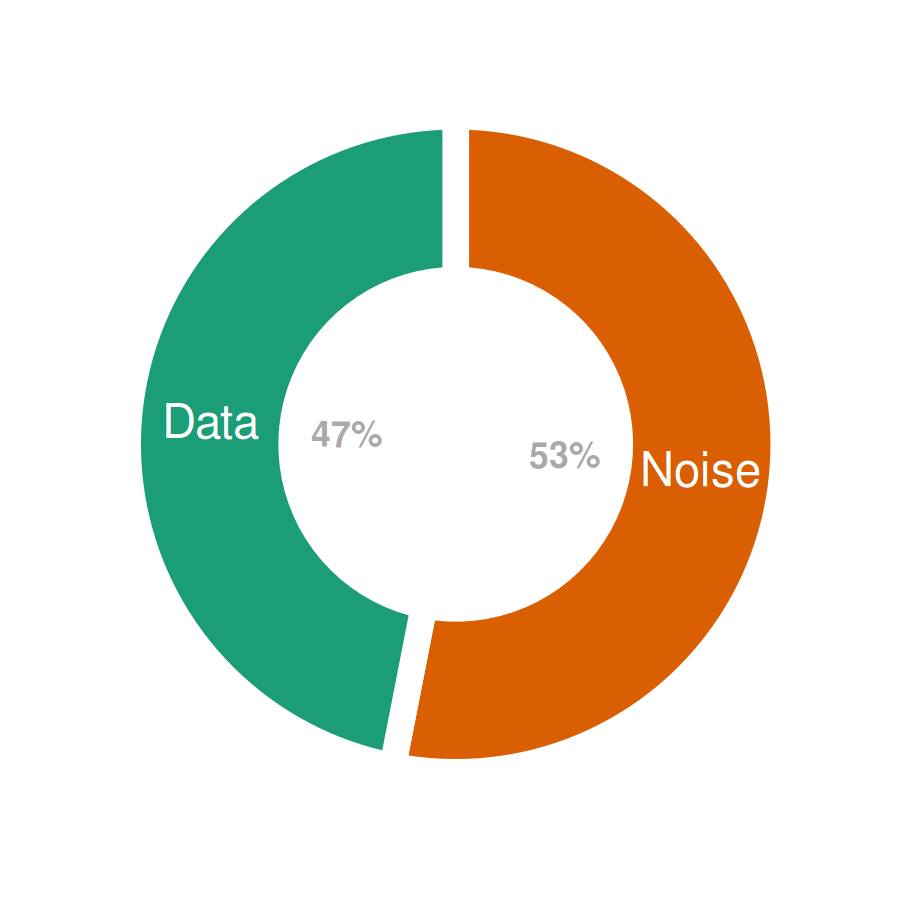
\includegraphics[trim={10 10 10 10},clip]{images/processing-error-signal.png}
  \caption{The share of noise present in the data from outside the field of measurement in the initial experiment.}
  \label{figure:processing:error:signal}
\end{marginfigure}

From the initial experiment, the noise due to the uncertain range of sensors was found to be much larger than expected.
It was observed that about 53\% of the total probe requests collected were from  outside the desired field of study.
As such the errors could be enormously reduced by simply filtering out the noise as shown in Figure \ref{figure:processing:error:signal}.
It was observed that the signal strength of the probe requests imparts valuable information on whether the probe request is generated by a device within the field of study or not.
Moreover, the amount of noise generated was found to be much greater in the data collected in a real world setting at UCL.
The experiment showed that the Mean Average Percentage Error when comparing the sensor counts to manual counts of pedestrians, was reduced from 736\% to  80\% just by removing signal strengths which were lower than -70dBm.
However, the problem with that methodology is the arbitrary nature of the threshold -70dBm which can vary widely based on the site conditions and over time.
A robust method was needed to calculate this threshold dynamically for each location at a particular time, and which was derived from the data itself rather than requiring external sources of information such as regular field surveys.

As discussed in Chapters \ref{chapter:literature} and \ref{chapter:collection} MAC randomisation is a major issue in the data.
It has arisen as a result of efforts to protect the privacy of the users of mobile devices, and it cannot be eliminated by simply collecting more data.
The belief that we should protect the privacy of mobile device users, also eliminates most of the intrusive techniques for collecting and processing data.
The technique of randomising MAC addresses has been used by the Windows Operating System on laptop computers for a long time, but it was brought mainstream when Apple Inc. introduced iOS 8 for their mobile devices in the fall of the 2015.
It was observed that there was a massive wave of adoption shortly after the release, but the trend stabilised as more and more of the market share was captured by Android devices, which were not randomising MAC addresses at the time.
The trend remained stable until the autumn of 2017, after which Android devices switched to randomisation techniques.
It is important to note that the randomisation methods were neither fool proof nor standardised, as showed by \citep{vanhoef2016}.
The problem of randomisation continued to intensify in 2017, and was attributed to the change in frequency that MAC addresses were randomised in a given time interval, thus increasing the proportion of local addresses in the dataset along with the total number of unique addresses.

\begin{figure*}
  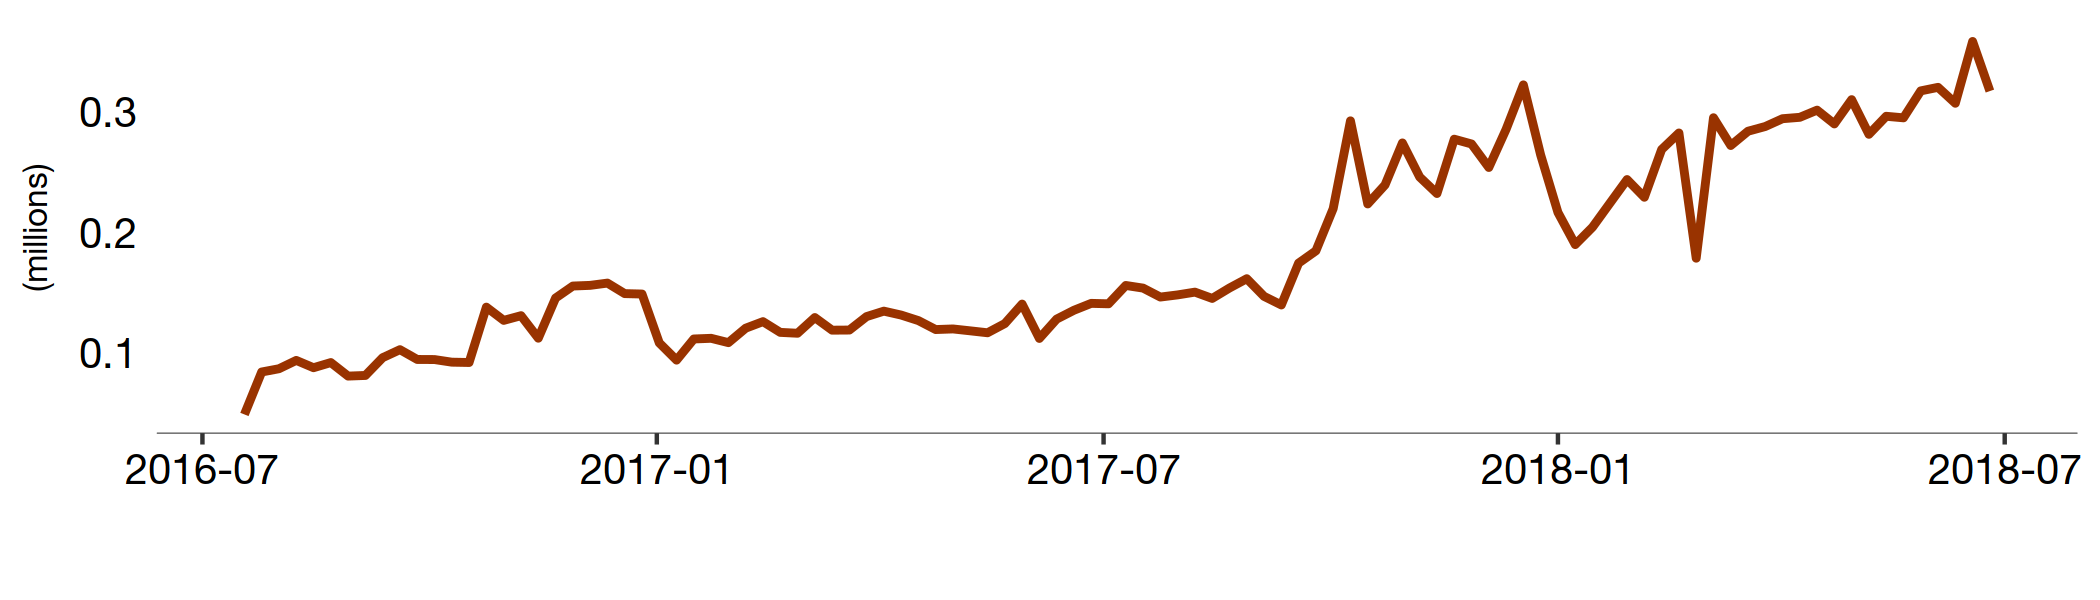
\includegraphics[trim={0 0 0 0},clip]{images/processing-error-randomisation.png}
  \caption{The long term effect of MAC randomisation on average weekly footfall estimated at sensors in Cardiff.}
  \label{figure:processing:error:random}
\end{figure*}

Figure \ref{figure:processing:error:random} shows the resulting ‘explosion’ in the average number of unique MAC addresses that occurred in September 2017 from a subset of data comprising of sensors in Cardiff.
It should be noted that the overall increase in the unique MAC addresses is not due to an increase of footfall at these locations.

In addition to causing problems generally in the data for longitudinal analysis, randomisation also causes issues at specific locations which have the potential for large amount of devices to dwell around them.
For example, seating areas in cafes / restaurants, bus stops, and phone shops around the sensors all cause huge overestimations of footfall when aggregated by unique MAC addresses.
It was therefore imperative that the method we devised should take both of these cases into consideration.


%------------------------------------------------------------------------------%
\subsection{Methodology}
%------------------------------------------------------------------------------%
Keeping the above considerations in mind, two methods to clean the Wi-Fi data and process them into footfall data were devised.
The first method uses signal strengths to filter out the noise originating from outside the field of view, and the second uses sequence numbers to group probe requests together instead of MAC addresses.

\vspace{1.5em}\noindent\textit{Filtering with Signal Strength}\vspace{0.5em}

\begin{marginfigure}
  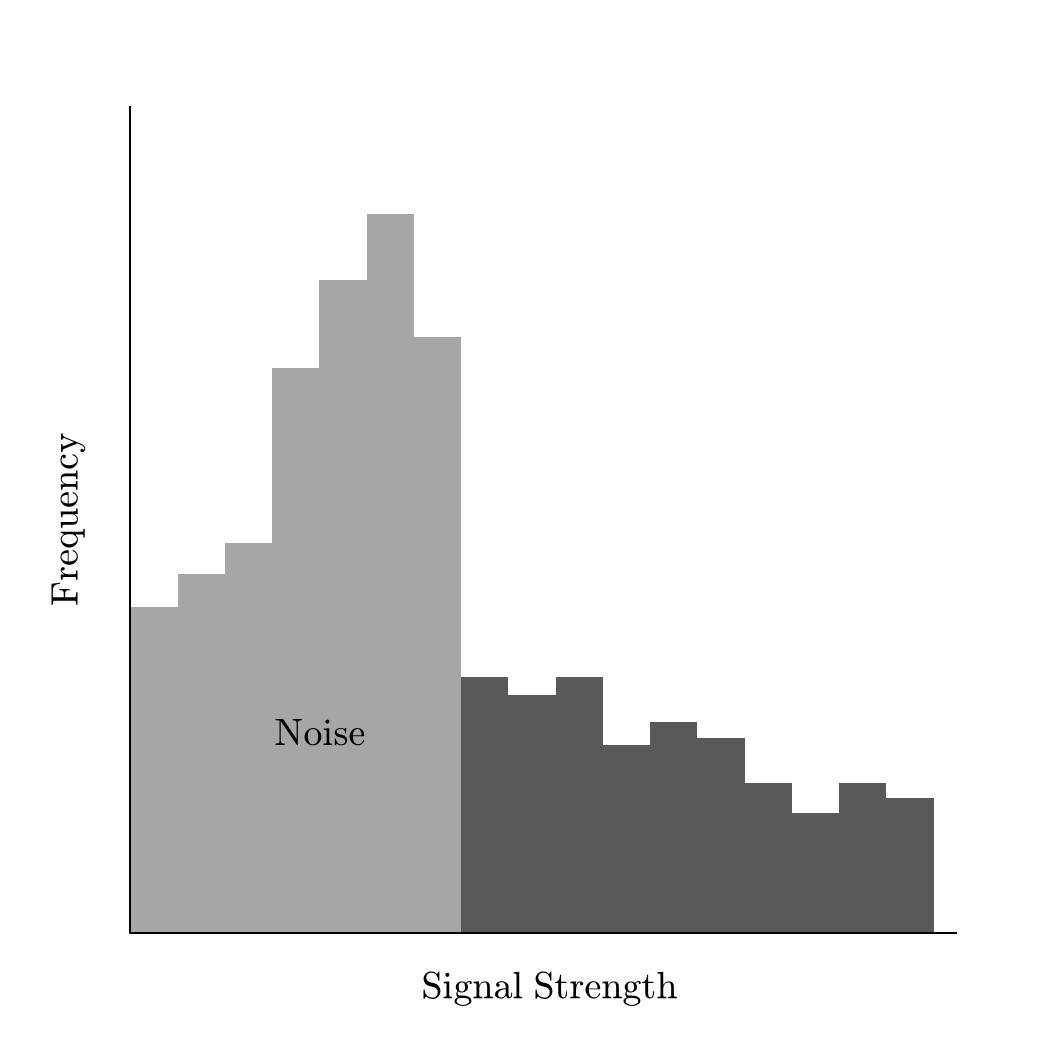
\includegraphics[trim={5 5 5 5},clip]{images/processing-method-signal.jpg}
  \caption{Thematic diagram showing the idea behind filtering using signal strength distribution.}
  \label{figure:processing:method:signal}
\end{marginfigure}

One of the clues that we used to estimate the distance between the mobile device and the sensor was the strength of the signal received by the sensor.
The first and obvious way to approach this problem was to try and establish a relationship between signal strength and distance.
Once established, the relationship was used to convert the measurement to distance, to set a distance threshold for every location, and finally to filter out the probe requests which were outside the distance threshold.
However as explained in section \ref{section:uncertainties}, this approach was found to be unfeasible.
The decay of signal strength with respect to distance is not always constant or linear and is fairly complex to model.
Moreover, the parameters with which these two were modelled together such as atmospheric conditions, the presence of obstructions between the source and the target, the material of these obstructions, and the strength of the signal (power level) of the source, vary widely across locations and across time as well.
This severely limits the ability to establish a simple conversion factor between reported signal strength and distance.
As such, a method which takes in to account all of these variables across the various locations needed to be devised.

Assuming that there are specific patterns in the way a sensor is installed at a location, it was expected that the data from around the sensor should reflect those patterns.
That is, in configurations where a specific source of background noise was at a constant distance, there should be a distinct pattern in the number of probe requests reporting signal strength corresponding to that distance.
For example, imagine a sensor in the middle of room such as in the initial experiment in this thesis, with devices in and outside the room.
In this case, assuming all the devices have roughly similar power levels, there should be a sudden drop in the signal strengths reported by the probe requests generated from outside the room when we look at their frequency distribution.
Alternatively, if there was a stationary source of noise such as a phone shop next to our sensor where hundreds of phones regularly send probe requests, there should  be a sharp rise in the of number of probe requests with reported signal strength corresponding to the distance between the sensor and the phone shop.
Both of these changes can be identified by the ‘breaks’ in the distribution of the signal strength data, as demonstrated schematically in Figure \ref{figure:processing:method:signal}.
Identification of these breaks in the data can be carried out using traditional one-dimensional clustering algorithms such as ‘jenks natural breaks’, ‘k-means’, ‘quantile’ and ‘hierarchical clustering’, etc.
 which are usually used to find the class intervals in data.
In simpler cases, the signal strength could be clustered into just ‘high’ and ‘low’ and the probes with low signal strengths could be ignored.

This approach has two primary advantages.
Firstly, it does not rely on a predetermined threshold that has to be calculated with a representative sample, which is not usually possible in time-series data with such variability.
Secondly, the methodology should apply for all the variations in micro-site conditions, since we are only looking for the relative breaks in the data and not for absolute values.
For example, if the sensor is located inside an enclosure and all the signals are of generally lower strength than usual, this method should still be able to find the distinction between the noise and the data from relatively near the sensors.
The disadvantages of this method is that it might not work in situations where there are multiple sources of noise around the sensor, as they do not create a distinct pattern in their distribution.

\vspace{1.5em}\noindent\textit{Clustering with sequence numbers}\vspace{0.5em}

There has been extensive research on extracting information about people from Wi-Fi probe requests in the past decade with feasible and favourable results.
However, all of the methods used in the research depends on the Wi-Fi data having a primary unique identifier: a MAC address.
When the MAC address is removed, or at least rendered non-unique, the established methods fail and cause significant risk to the infrastructure and commercial applications built around Wi-Fi data.
As was shown in Chapter \ref{chapter:literature}, various methods have been devised to overcome this anonymisation process including, but not limited to,

\begin{itemize}[rightmargin=2em, leftmargin=2em]
  \itemsep-0.25cm
  \item \textit{Profiling Manufacturers}: estimating the device model information from a known dataset of manufacturers and device behaviours \citep{martin2016}
  \item \textit{Scrambler attack}: using another small part of the physical layer specification for Wi-Fi \citep{vo2016, bloessl2015}
  \item \textit{Timing attack}: where the packet sequence information along with information elements present in the probe request frame is used \citep{matte2016, cheng2016}. 
\end{itemize}

A combination of these methodologies has been proven to produce de-anonymised globally unique device information\cite[-4cm]{vanhoef2016, martin2017}.
Although these approaches are effective, sometimes even up to 90\%, they usually result in a serious risk of breach of privacy of the users of the mobile devices by revealing their MAC addresses or by crossing ethical lines by tricking the devices into sending more information than they would ordinarily include in a probe request.
Moreover, these risks are considered vulnerabilities by the computer security industry and are usually ‘patched’ in a reasonable amount of time, hence reducing their effectiveness in long term.
As a consequence, it was necessary to explore methodologies for estimating the number of unique mobile devices from a set of anonymised probe requests, without the need to reveal their original device information.

Although the sequence number of the packet is not strictly unique to a particular mobile device, it was hypothesised that they can be used to estimate the number of unique devices.
\citet{vanhoef2016} used optional information present in the probe requests - Information Elements (IE) - along with the sequence numbers to successfully fingerprint the devices.
This approach has become increasingly difficult as mobile phone manufacturers, especially Apple, have severely limited the number of information elements in the probe requests to curb such finger printing process.
This problem affects established commercial solutions using Wi-Fi probe requests such as Blix, Walkbase, Euclid Analytics, and RetailNext etc.
These companies solve the randomisation by combining Wi-Fi data with other sources of data such as cameras, lasers or infrared counters, but this is not possible for our research.
More recently, another solution to the problem was  proposed by \citet{hong2018}\cite{hong2018} whereby a \textit{Hidden Markov Models} based trajectory inference algorithm was deployed.
Unfortunately the research was limited to enclosed, exit-controlled public spaces such as shopping malls and railway stations, and therefore does not translate well to the open retail high streets studied in this thesis.
As such, a novel method to suit the context of this research was devised.

The first approach taken was to establish a ‘factor of randomisation’: the ratio of the total number of randomised probe requests emitted  to the number of unique MAC addresses in them.
This factor was then used to adjust the counts when aggregating the randomised probe requests.
As explained in section \ref{section:uncertainties}, the rate of probe request generation is highly variable and an approach which assumed a constant and stable rate of probe requests, was therefore not feasible.
Moreover, since software and specification change frequently, it was surmised that this method was not feasible in the long-term.
It was necessary to create a more general approach independent of the device model or manufacturer.

\begin{marginfigure}
  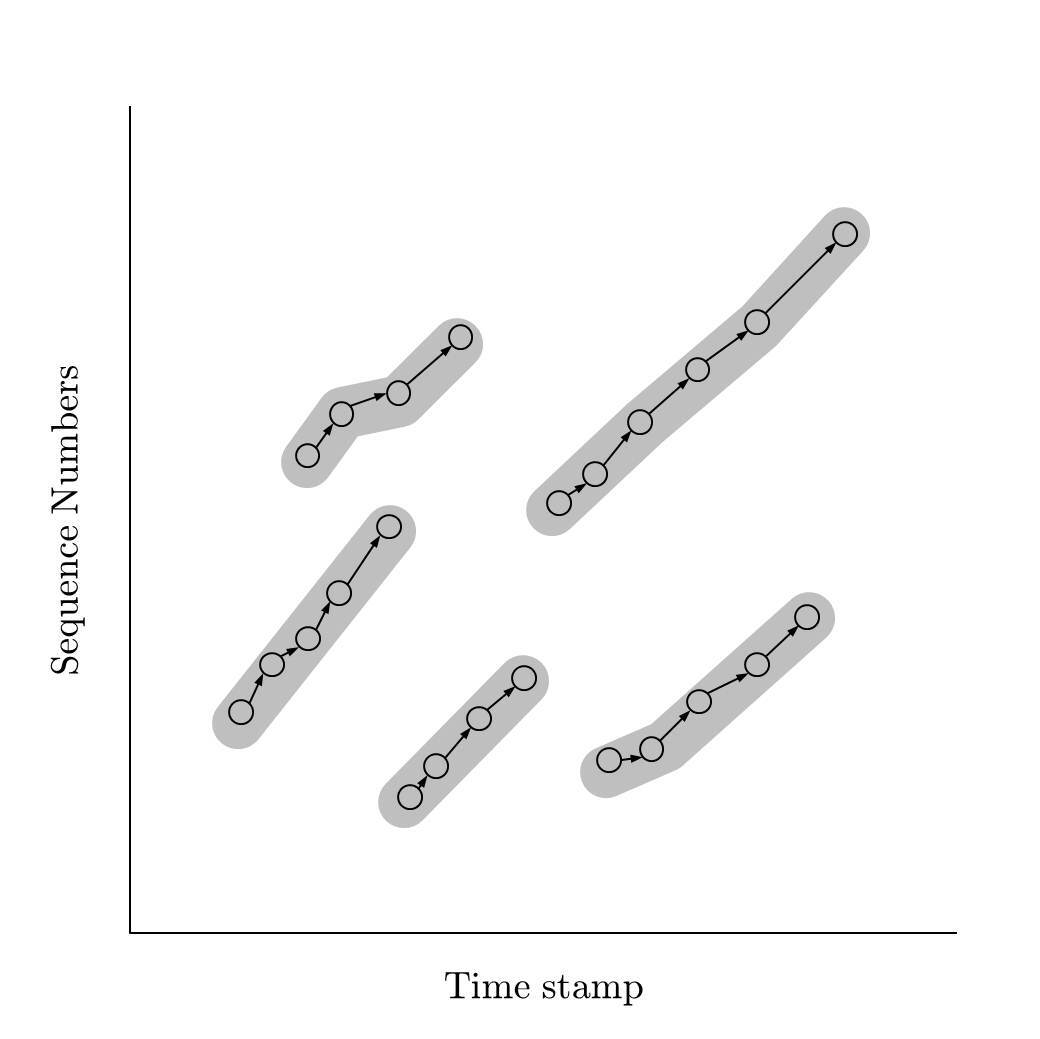
\includegraphics[trim={5 5 5 5}, clip]{images/processing-method-sequence.jpg}
  \caption{Thematic diagram showing the idea behind grouping sensors using their sequence numbers.}
  \label{figure:processing:method:sequence}
\end{marginfigure}

Resulting from the initial experiments explained in section \ref{section:intial:experiments}, it was found that OUI and the sequence number of the probe request were the most promising information to achieve this.
It was also observed that, when plotted against time stamps, sequence numbers show distinct streak patterns which could be isolated as single unique devices.
Since only one probe request can be received at a time, it was possible to link them using a graph-based algorithm as illustrated in Figure \ref{figure:processing:method:sequence}.
Such an algorithm would create a graph with the randomised probe requests whereby the nodes were the probe requests themselves.
The edges were created between the nodes based on the following rules:

\begin{enumerate}[rightmargin=3em, leftmargin=3em] 
  \itemsep-0.5em
  \item A link could go only forward in time.
  \item A link could go from low to high sequence numbers. 
  \item A link could exist between nodes with a maximum time difference of $\alpha$ - time threshold.
  \item A link could exist between nodes with a maximum sequence number difference of $\beta$ - sequence threshold.
  \item A node could have only one incoming link and one outgoing link, which is the shortest of all such possible links.
\end{enumerate}

The first two rules arise from how the Wi-Fi data collection process works.
The third and fourth rules create a kind of 2 dimensional moving window within which all the links are connected.
The final rule simplifies the graph into strands of unique devices based on the assumption that the closest points within a window belong together.
This, of course, will not work accurately when there are intersections between these strands.
This solution could be made more accurate by calculating angular changes similar to techniques used in creating ‘dual networks’ in roads\cite{masucci2014}, but could disproportionately increase the amount of processing needed.
Hence for this research, the former method which uses the shortest link was used.

After simplifying the graph conceptually, each connected component corresponds to a device generating probe requests periodically with increasing sequence numbers.
 A unique identification number was then assigned to the nodes based on the connected component of the graph they belonged to.
This unique identifier was then used in place of MAC addresses for the aggregation of the anonymised probe requests.
As discussed in section \ref{wifi-as-source-of-data}, the sequence numbers do not always increase as they get reset after 4096; thus, this method can lead  to multiple unique identifiers being reported for a single device.
This can be potentially solved by treating sequence numbers as a ‘ratio’ scale, while calculating distances between probe requests.
Since a sample consisting of randomised probe requests sent by "Google" devices in the data collected from the initial experiments showed that only 0.5\% of the sample had their sequence number reset in a given period, this effect has been deemed inconsequential and ignored in this research.

\vspace{1.5em}\noindent\textit{Calibrating with Ground Truth}\vspace{0.5em}

Since proportion of mobile device ownership was an external uncer- tainty to this study and could arise from variety of spatio-temporal and demographic factors, the study aimed to solve the uncertainty by using a manual sample count at each location.
An adjustment factor or an ‘offset’ was calculated for each location by comparing the sensor-based counts and ground truth, similar to what was undertaken in the beginning of the project.
This adjustment factor was then used to adjust the rest of the data reliably to reflect the ground truth in absolute numbers.
On a project with a large scope, such as the Smart Street Sensor project, since this calibration applies in addition to the other methodologies, in addition to increasing accuracy of measurement in the short time, they can be carried out periodically at chosen locations to improve the quality of estimation over a long time.

The three methods – signal strength filtering, sequence number clustering, and manual calibration - together provide a unified methodology for converting the Wi-Fi probe requests into footfall.
But the methods need empirical experiments for a successful implementation with real- world data.
For example, the signal strength methodology we need to find the most suitable one dimensional clustering algorithm and for the sequencing method the values of threshold need to be calculated.
These questions were answered by applying the methods on the data collected in the experiments and pilot study as detailed in the upcoming sections.

%------------------------------------------------------------------------------%
\subsection{Oxford Street Experiment}
%------------------------------------------------------------------------------%

The primary aim of the initial experiment conducted on Oxford Street, London was to collect data to validate the filtering and clustering meth- ods against the scale and complexity of an open public area.
It was also aimed at finding the algorithm which was best suited for the one dimensional classification of signal strengths as either ‘low’ or ’high’, in order to filter out the background noise.

The first step was to create a base line count or ‘raw count’ without any cleaning procedures, whereby the probe requests were aggregated by their MAC addresses for every minute.
This generated a continuous, minute-by-minute count of the number of people estimated to be near the sensor.
It was assumed that each MAC address corresponded to a mobile device and hence a pedestrian.
This preliminary ‘footfall’ count was then compared to the actual number of pedestrians recorded manually to check for robustness.
The statistic - Mean Absolute Percentage Error (MAPE) – was used as a measure of robustness of the count, since it provided a simple and quick idea of how much the pair of time series data differed from each other.
MAPE generally does not work with datasets with a significant number of data points which are not known, or those which contain zero values; however, because of the busy nature of the survey location, there were no such intervals without any footfall.

It was observed that the MAPE in these raw counts, when compared to the actual ground truth, was around 425\%.
This confirmed the presence of a large amount of noise in the data which may have been generated by the sources of uncertainties discussed in section \ref{section:uncertainties}.
It also demonstrated the need for filtering the data before aggregating them into footfall.

\begin{table}
  \footnotesize
  \caption{Comparison of clustering algorithms with a sample of 40000 probe requests}
  \centering
  \begin{tabular}{lcc} 
    \toprule
     Algorithm				      	& Time (s)& MAPE\\
    \midrule
     Quantile				        	& 0.002 	&  27 \% \\
     K-Means			 	        	& 0.007 	& -23 \% \\
     Hierarchical Clustering	& 172.520	&  -9 \% \\
     Bagged Clustering 		  	& 0.135 	& -30 \% \\
     Fisher 				        	& 3.034 	& -30 \% \\
     Jenks Natural Break 	   	& 556.279	& -30 \% \\
     \bottomrule
  \end{tabular}
  \label{table:processing:oxst:classification}
\end{table}

The probe requests were then classified as ‘high signal strength’ or ‘low signal strength’ using various one dimensional clustering algorithms.
The algorithms used were as k-means, quantile, hierarchical clustering, bagged clustering, fisher and jenks natural breaks with the number of clusters set as 2.
Due to the processor-intensive nature of some of these algorithms, only a sample of 40,000 probe requests were selected for this benchmarking exercise.
For each exercise, the resulting probe requests were filtered only for those with high signal strength, and rest were discarded.
As before, the filtered probe requests were then converted into footfall counts by aggregating them based on their MAC addresses, and subsequently compared to the manual footfall counts.

Two metrics were collected for each clustering algorithm: the time it took to classify all the data points in the sample, and the amount of MAPE in the resulting footfall estimates.
The results are shown in Table \ref{table:processing:oxst:classification}.
It was found that out of all algorithms, hierarchical clustering and jenks natural break provided the least amount of errors.
However, these two algorithms were designed to identify class intervals in much smaller datasets and were extremely resource intensive for practical use with a larger dataset.
It was also found that the k-means algorithm gave the quickest result with the lowest MAPE, closely followed by the quantile algorithm.
The cut-off point, or threshold, for the collected data with which we could classify the probe requests as high and low was found to be -71 dBm, using the k-means algorithm.
When the data were aggregated after this filtration process to remove all the probes with a ‘low’ signal strength, it resulted in a footfall count with a MAPE of 30\%.
This was extremely encouraging considering the magnitude of improvement.
However, it was not certain if this filtering process was  removing noise only from outside, or if it had any kind of independence from the configuration of the sensor at the location.
These concerns needed to be addressed with a larger survey with multiple locations, as discussed in the pilot study.

\begin{figure*}
  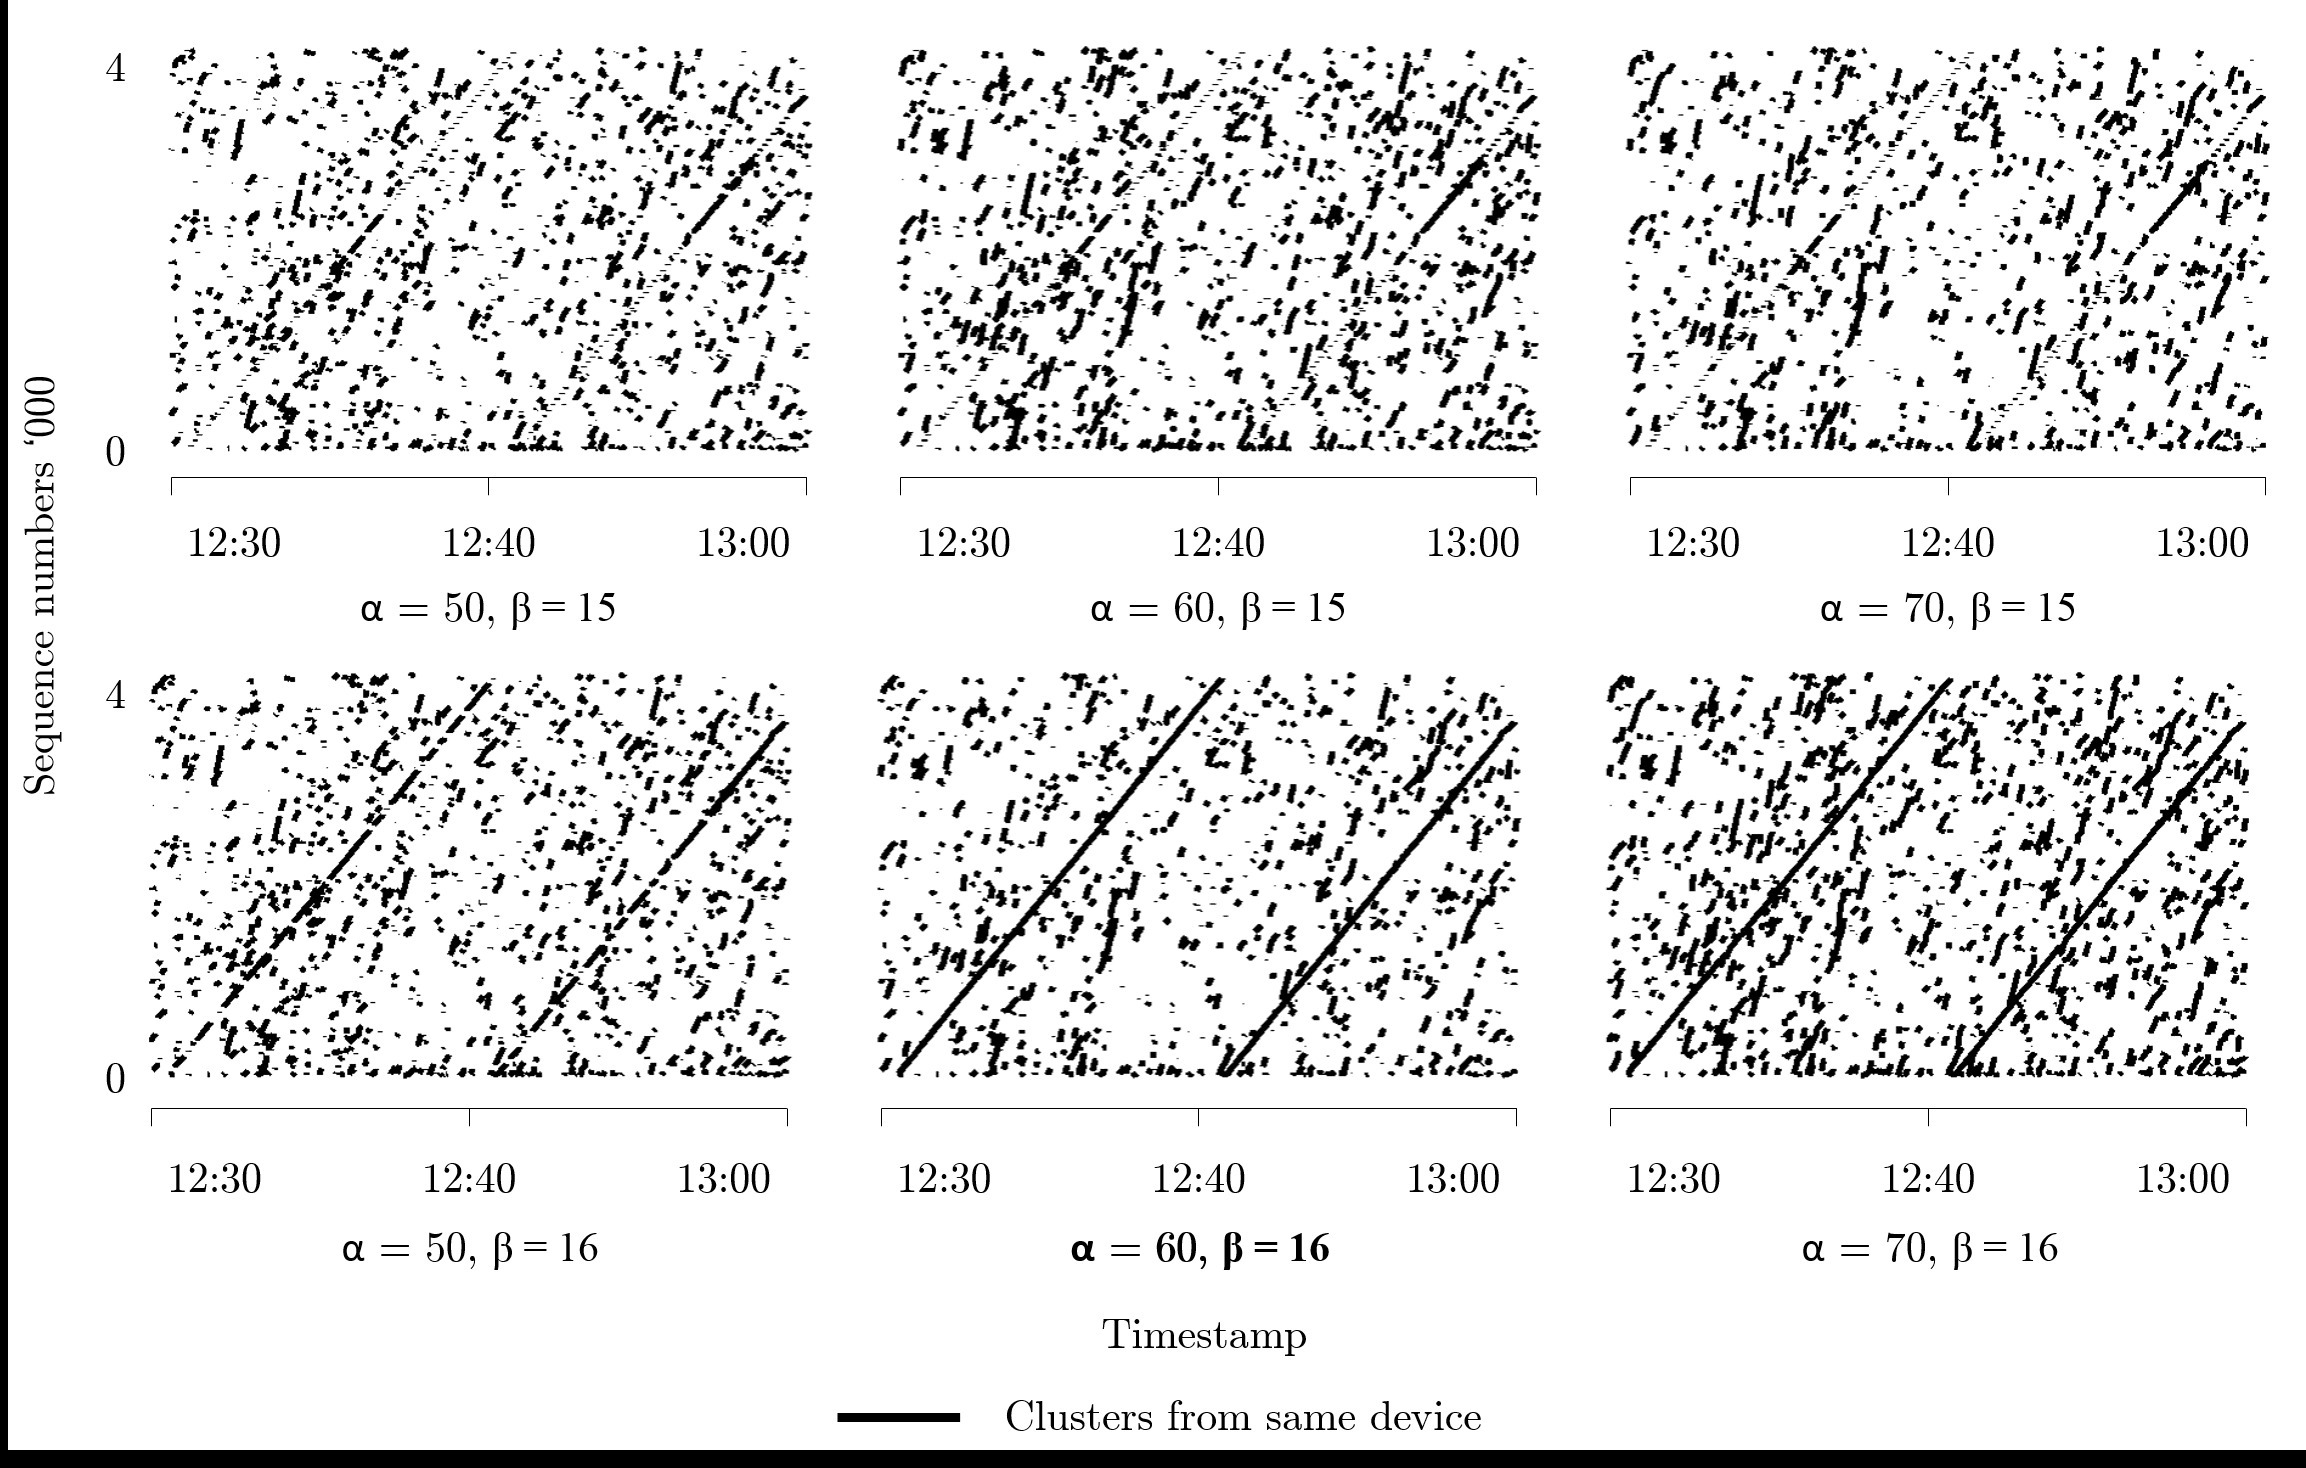
\includegraphics[trim={1 1 1 1},clip]{images/processing-oxst-clusters.jpg}
  \caption{Finding the optimum time threshold $\alpha$ and sequence threshold $\alpha$ through trial and error.}
  \label{figure:processing:oxst:clusters}
\end{figure*}

With the filtering method validated, the next step was to identify the probe requests which were generated by the same device irrespective of the MAC randomisation using their sequence numbers.
The graph theory based algorithm defined earlier was employed and each local probe request was assigned an alternative unique identifier or signature independent of their the MAC addresses.
Since a baseline for the nature or frequency of the MAC address randomisation process could not be established, the surveyor’s mobile device was used as a reference.
As the surveyor’s device was being actively used to count pedestrians with its Wi-Fi module kept active without establishing connection to any network, it was known that the device was continuously probing for new networks.
Moreover, since the screen of the device was switched on with constant taps the frequency of these probe requests were higher than normal.
It was also known that the OUI of the device corresponded to the vendor - ’Google’ – and that the device was regularly randomising its MAC address.
All in, it served as an excellent reference point with which it was possible to determine if the clustering method has worked.

\begin{figure}
  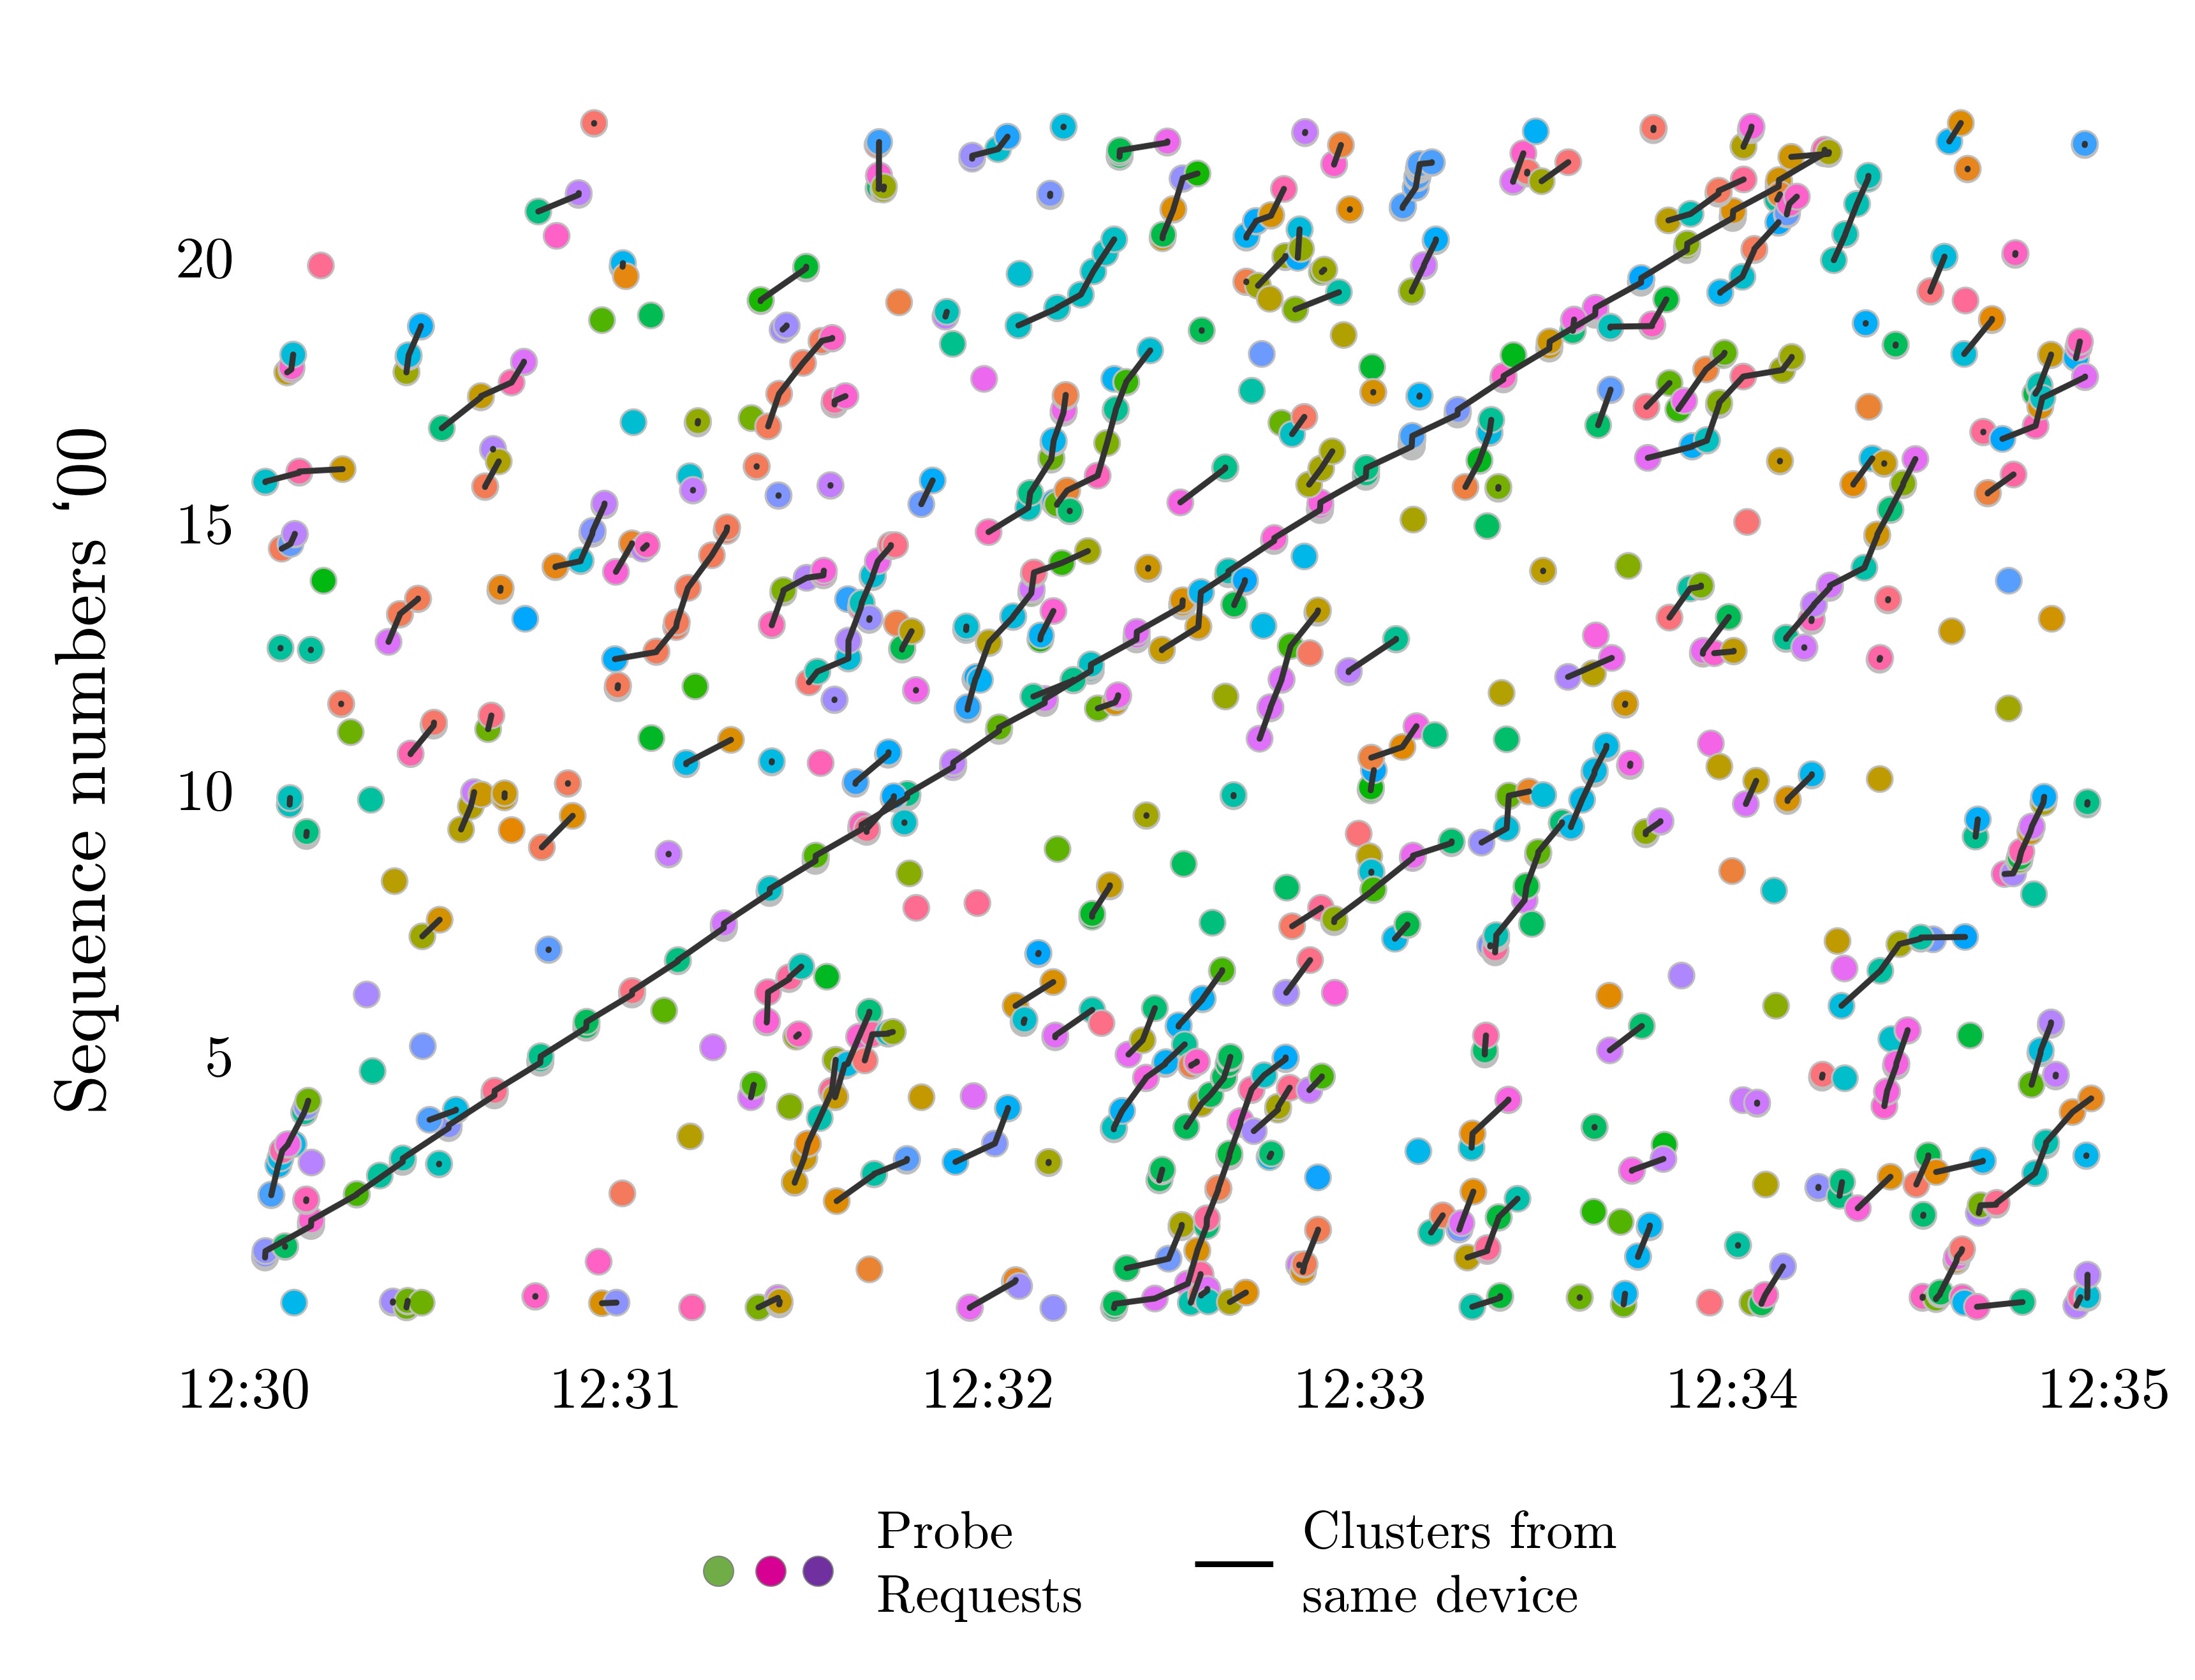
\includegraphics[trim={3 3 3 3},clip]{images/processing-oxst-fingerprinting.jpg}
  \caption{Sample showing the result of sequence numbers based clustering algorithm on data collected at Oxford Circus, London.}
  \label{figure:processing:oxst:fingerprinting}
\end{figure}

The algorithm required two parameters which needed to be determined empirically - sequence threshold and time threshold - which was done using trial and error as described below.
The clustering process was done repeatedly with increasing values for both thresholds in increments of 1, and for each increment, the resulting clusters were  examined to see if the data from the reference device were clustered into one device.
The minimum possible time and sequence thresholds at which the algorithm clustered the reference device properly without over clustering the other probe requests, or under clustering as multiple devices, is illustrated in Figure \ref{figure:processing:oxst:clusters}.
It can be observed that the threshold for time $\alpha$ and the threshold for sequence numbers $\beta$, are 16 seconds and 60 respectively.

Figure \ref{figure:processing:oxst:fingerprinting} shows the results of this clustering process on a small set of randomised probe requests collected in this experiment.
The probe requests with different randomised MAC address are shown by the coloured dots and the lines joining them show that those probe requests were clustered together by the algorithm and are most likely generated by the same device.
The data were finally aggregated as before, but with this device’s signature rather than the local MAC addresses.
This resulted in a footfall count with a MAPE of -18\% compared to the manual count.
It is important to notice that this clustering was undertaken on top of the signal strength filtering, and only for the probe requests with randomised MAC addresses.
A comparison of minute by minute counts resulting from different filtering processes along with the ground truth is shown in Figure \ref{figure:processing:oxst:results}, and illustrates the promising effectiveness of the methods.

\begin{figure}
  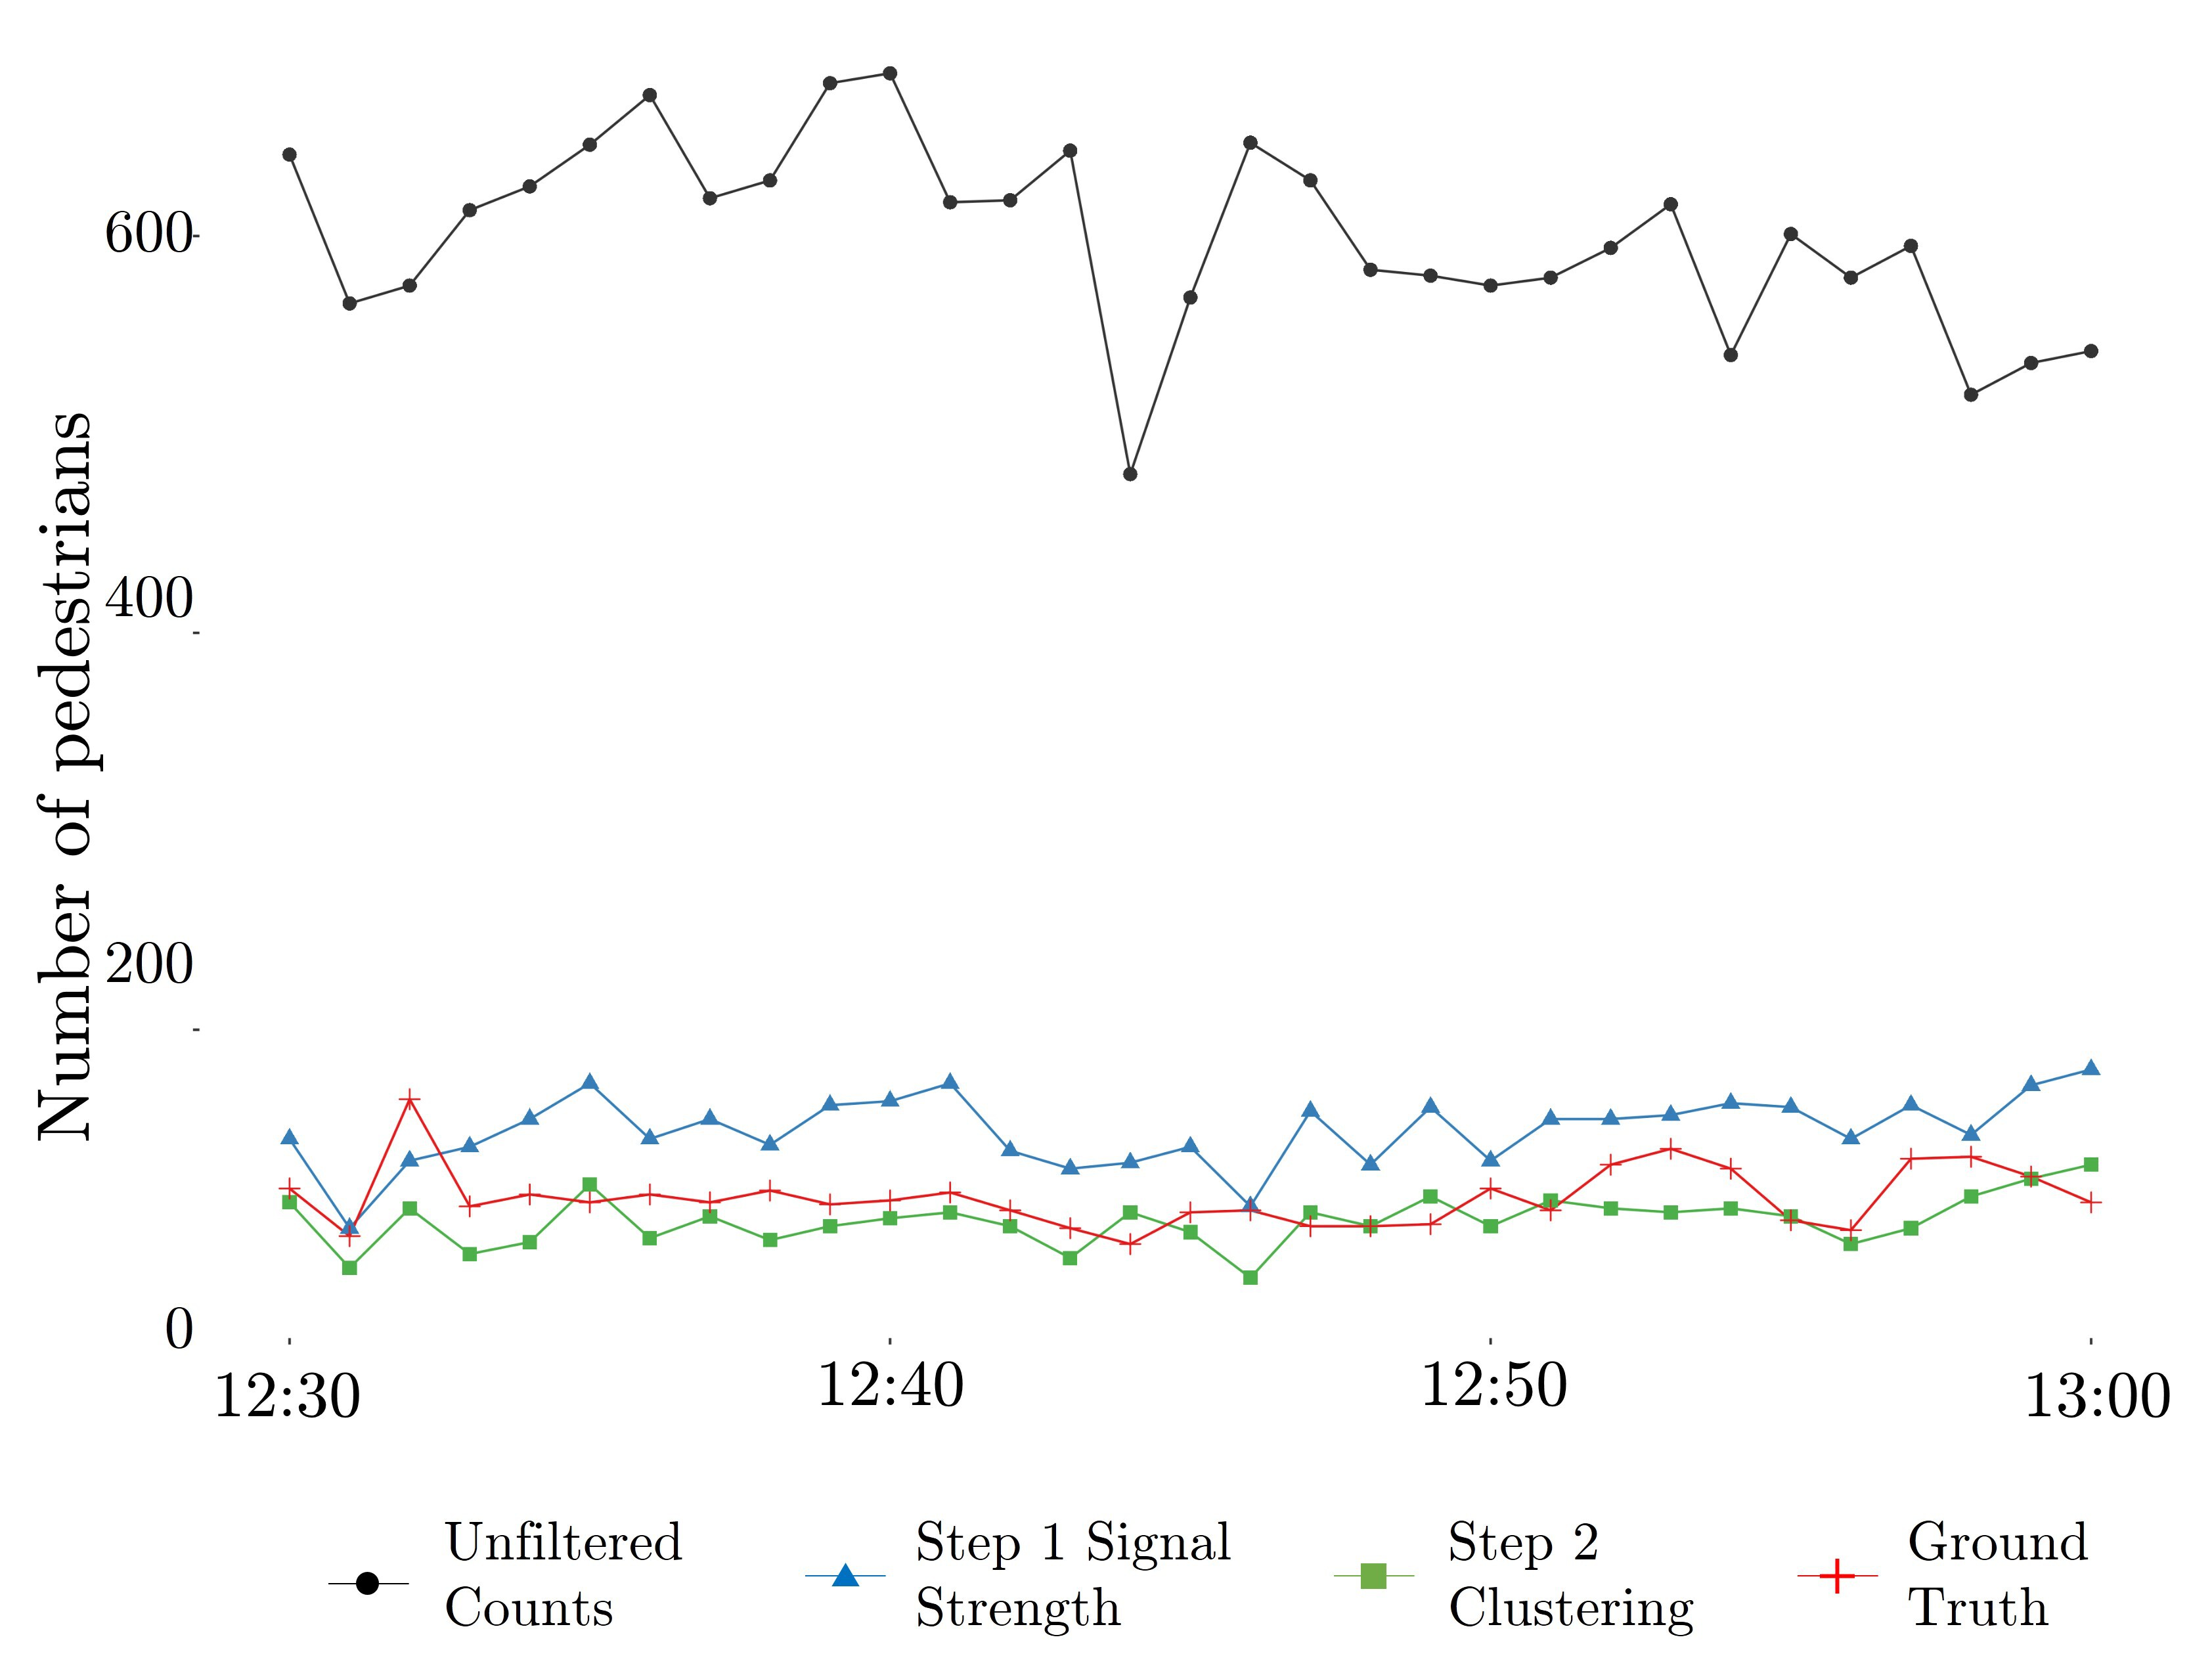
\includegraphics[trim={3 3 3 3},clip]{images/processing-oxst-results.jpg}
  \caption{A comparison of estimated footfall at Oxford Circus during various stages of filtering with the actual manual counts.}
  \label{figure:processing:oxst:results}
\end{figure}

To summarise, the data from the initial experiments suggest that both filtering using signal strength and the clustering using sequence numbers worked well on complex, real world data and resulted in fairly accurate pedestrian counts with a MAPE of 20\%.
It was also found that ‘k-means’ and ‘quantile’ are the best algorithms for clustering signal strengths, and the optimum thresholds for time and sequence numbers for the clustering algorithm were around 16 and 60 respectively.

%------------------------------------------------------------------------------%
\subsection{Pilot Study}
%------------------------------------------------------------------------------%

With encouraging results from the initial experiment, the next step was to check if the methods worked on the various locations where sensors were installed in different configurations using the data from the pilot study.
The distribution of the signal strengths of all the probe requests collected at each location were created and were compared to the corresponding sensor configurations at these locations.
When visualised as density plots as shown in Figure \ref{figure:processing:pilot:signal}, they show a clear relationship between the distribution of the signal strength and the distance and complexity of  the source of noise at each location.
It was observed that when there is clear distinction between the source of noise where stationary devices were generating randomised local probe requests, the signal strength distribution shows a clear distinction between high and low values.
For example, at location 5 where the noise is generated by a phone shop next door, a significant spike in the number of probe requests generated with similar low signal strength was also reported.
Whereas, location 2 - a restaurant located  next to a public square  with seating on both sides   of the sensor - shows no such discernible distinction of any sort.
This demonstrates that filtering using signal strength works, but at the same time depends heavily on the assumption that the sensor is installed in such a way that the field of measurement is clearly ‘visible’ in terms of distance from it.
Figure \ref{figure:processing:pilot:signal} confirmed the intuition that data collected at location 2 and 4 would be harder to clean than the ones collected at locations 1, 3 and 5.
The signal strength threshold, calculated using k-means algorithm, for all the locations except for 2 were between -72 dBm and -70 dBm - very much in line with the findings of the initial experiment.
This also introduced the possibility that -70dBm could be used as a rule of thumb for filtering noise at a general location unless it faced specific challenges like location 2.
It is important to note that as the aim was  to compare the counts with manual counts, the data used  to calculate the threshold pertains only to the time when manual counting was undertaken at these locations.
Like before, the data were aggregated using MAC addresses after removing points with low signal strength and compared with manual counts.
The results are shown in Table \ref{table:processing:pilot:results}.
In this exercise probe requests with MAC addresses which repeated within a 15 minute window were also removed.

\begin{figure*}
  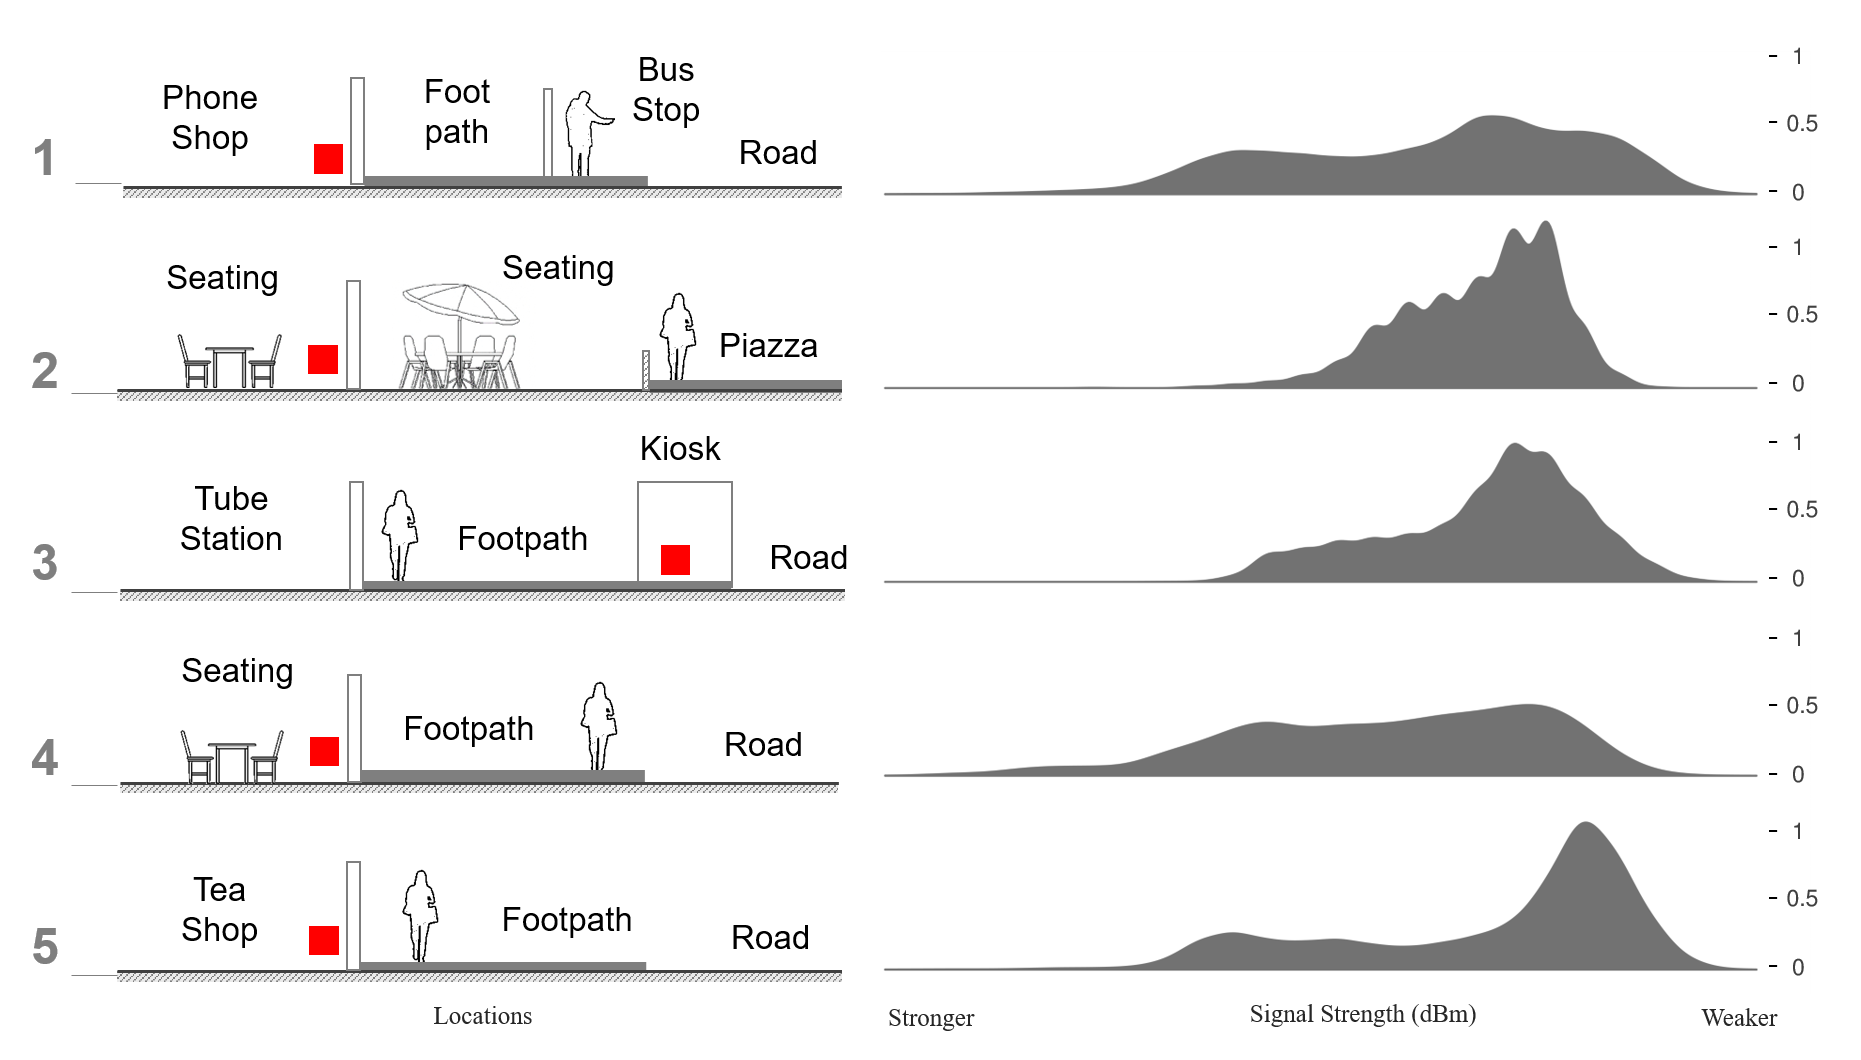
\includegraphics{images/processing-pilot-signal.png}
  \caption{Distribution of signal strengths at locations covered under the pilot studies along with the corresponding configurations of the sensors.}
  \label{figure:processing:pilot:signal}
\end{figure*}

We observed that the MAPE at locations 1,4 and 5 was reduced to -19\% to 150\% from the original 250\% to 500\%, making this an ideal candidate for a quick and easy cleaning procedure for most practical applications.
Locations 2 and 3 were found to be particularly tricky: the former had the propensity to overestimate the footfall, and the latter underestimated it.
This could also be attributed to the configuration of the sensor at the particular location.
Location 3 was particularly interesting as it is the only location with no source of stationary noise and almost all the probe requests collected at this location should be coming from genuine footfall.
It was observed that the filtering needs to be less aggressive in locations without any obvious source of noise to prevent underestimating footfall at these locations.

\begin{centering}
\begin{table}
\footnotesize
\caption{Results of footfall estimation at each location as Mean Absolute Percentage Error (MAPE) after each step of the filtering process.}
{\begin{tabular}{ccccccc} 
\toprule
& Signal    & Adjustment & MAPE      & MAPE      & MAPE       & MAPE final \\
Sensor  & threshold & factor     & before    & after     & after    & adjusted\\
& (-dBm)    &            & filtering & filtering & clustering & count\\
&           &            & (\%)      & (\%)      & (\%)       & (\%)\\
\midrule
1 & -70 & 1.25 & 259 &  22 & -13 &  9 \\
2 & -74 & 0.51 & 928 & 396 & 206 & 55 \\
3 & -72 & 1.60 &  87 & -19 & -31 & 10 \\
4 & -70 & 0.88 & 498 & 142 &  52 & 33 \\
5 & -72 & 0.80 & 473 &  84 &  38 & 11 \\
\bottomrule
\end{tabular}}
\label{table:processing:pilot:results}
\end{table}
\end{centering}

The next step was to test the sequence number based clustering al- gorithm on these locations.
The sequence number clustering algorithm was run on the local MAC addresses to cluster the probe requests; the resulting device signatures were used to aggregate them into footfall counts.
The results showed that this process further reduced the MAPE to almost 13\% - 300\% on all the sensors with a clean configuration.
Locations 3 and 2 were still outliers due to their complex configurations.
The final step was to test the simple manual calibration process: an adjustment factor was calculated for each location as the ratio between footfall estimated from the sensor after processing and the actual pedestrian counts.
This adjustment factor was used to adjust the counts.
It is important to note that the adjustment factor and MAPE were calculated using an interval from a different location than the manual counts.
This process further reduces the MAPE to 10\% - 50\% while taking care of the over-counting problem in Location 3.
Location 2 is still not as accurate as the MAPE after all the processing that was done, which highlights the limitations of the methods discussed.
Figure \ref{figure:processing:pilot:final} shows the effectiveness of these cleaning procedures at each location.

To summarise, the pilot study confirmed the findings from the initial experiment by showing that the signal strength based filtering is effective and provides a quick and easy way to clean out the noise, when used along with the sequence numbers based finger-printing technique.
It also demonstrated that the sensors with no discernible  stationary  source  of  noise  tend to under-count pedestrians, and therefore require that calibration is done using manually collected data.
In contrast, sensors with seating next to them significantly over-count footfall.
However, the study also proved that through the process of cleaning, the counting errors can be reduced substantially resulting in the sensor based counts being accurate within 10\% of the ground truth.

\begin{figure*}
  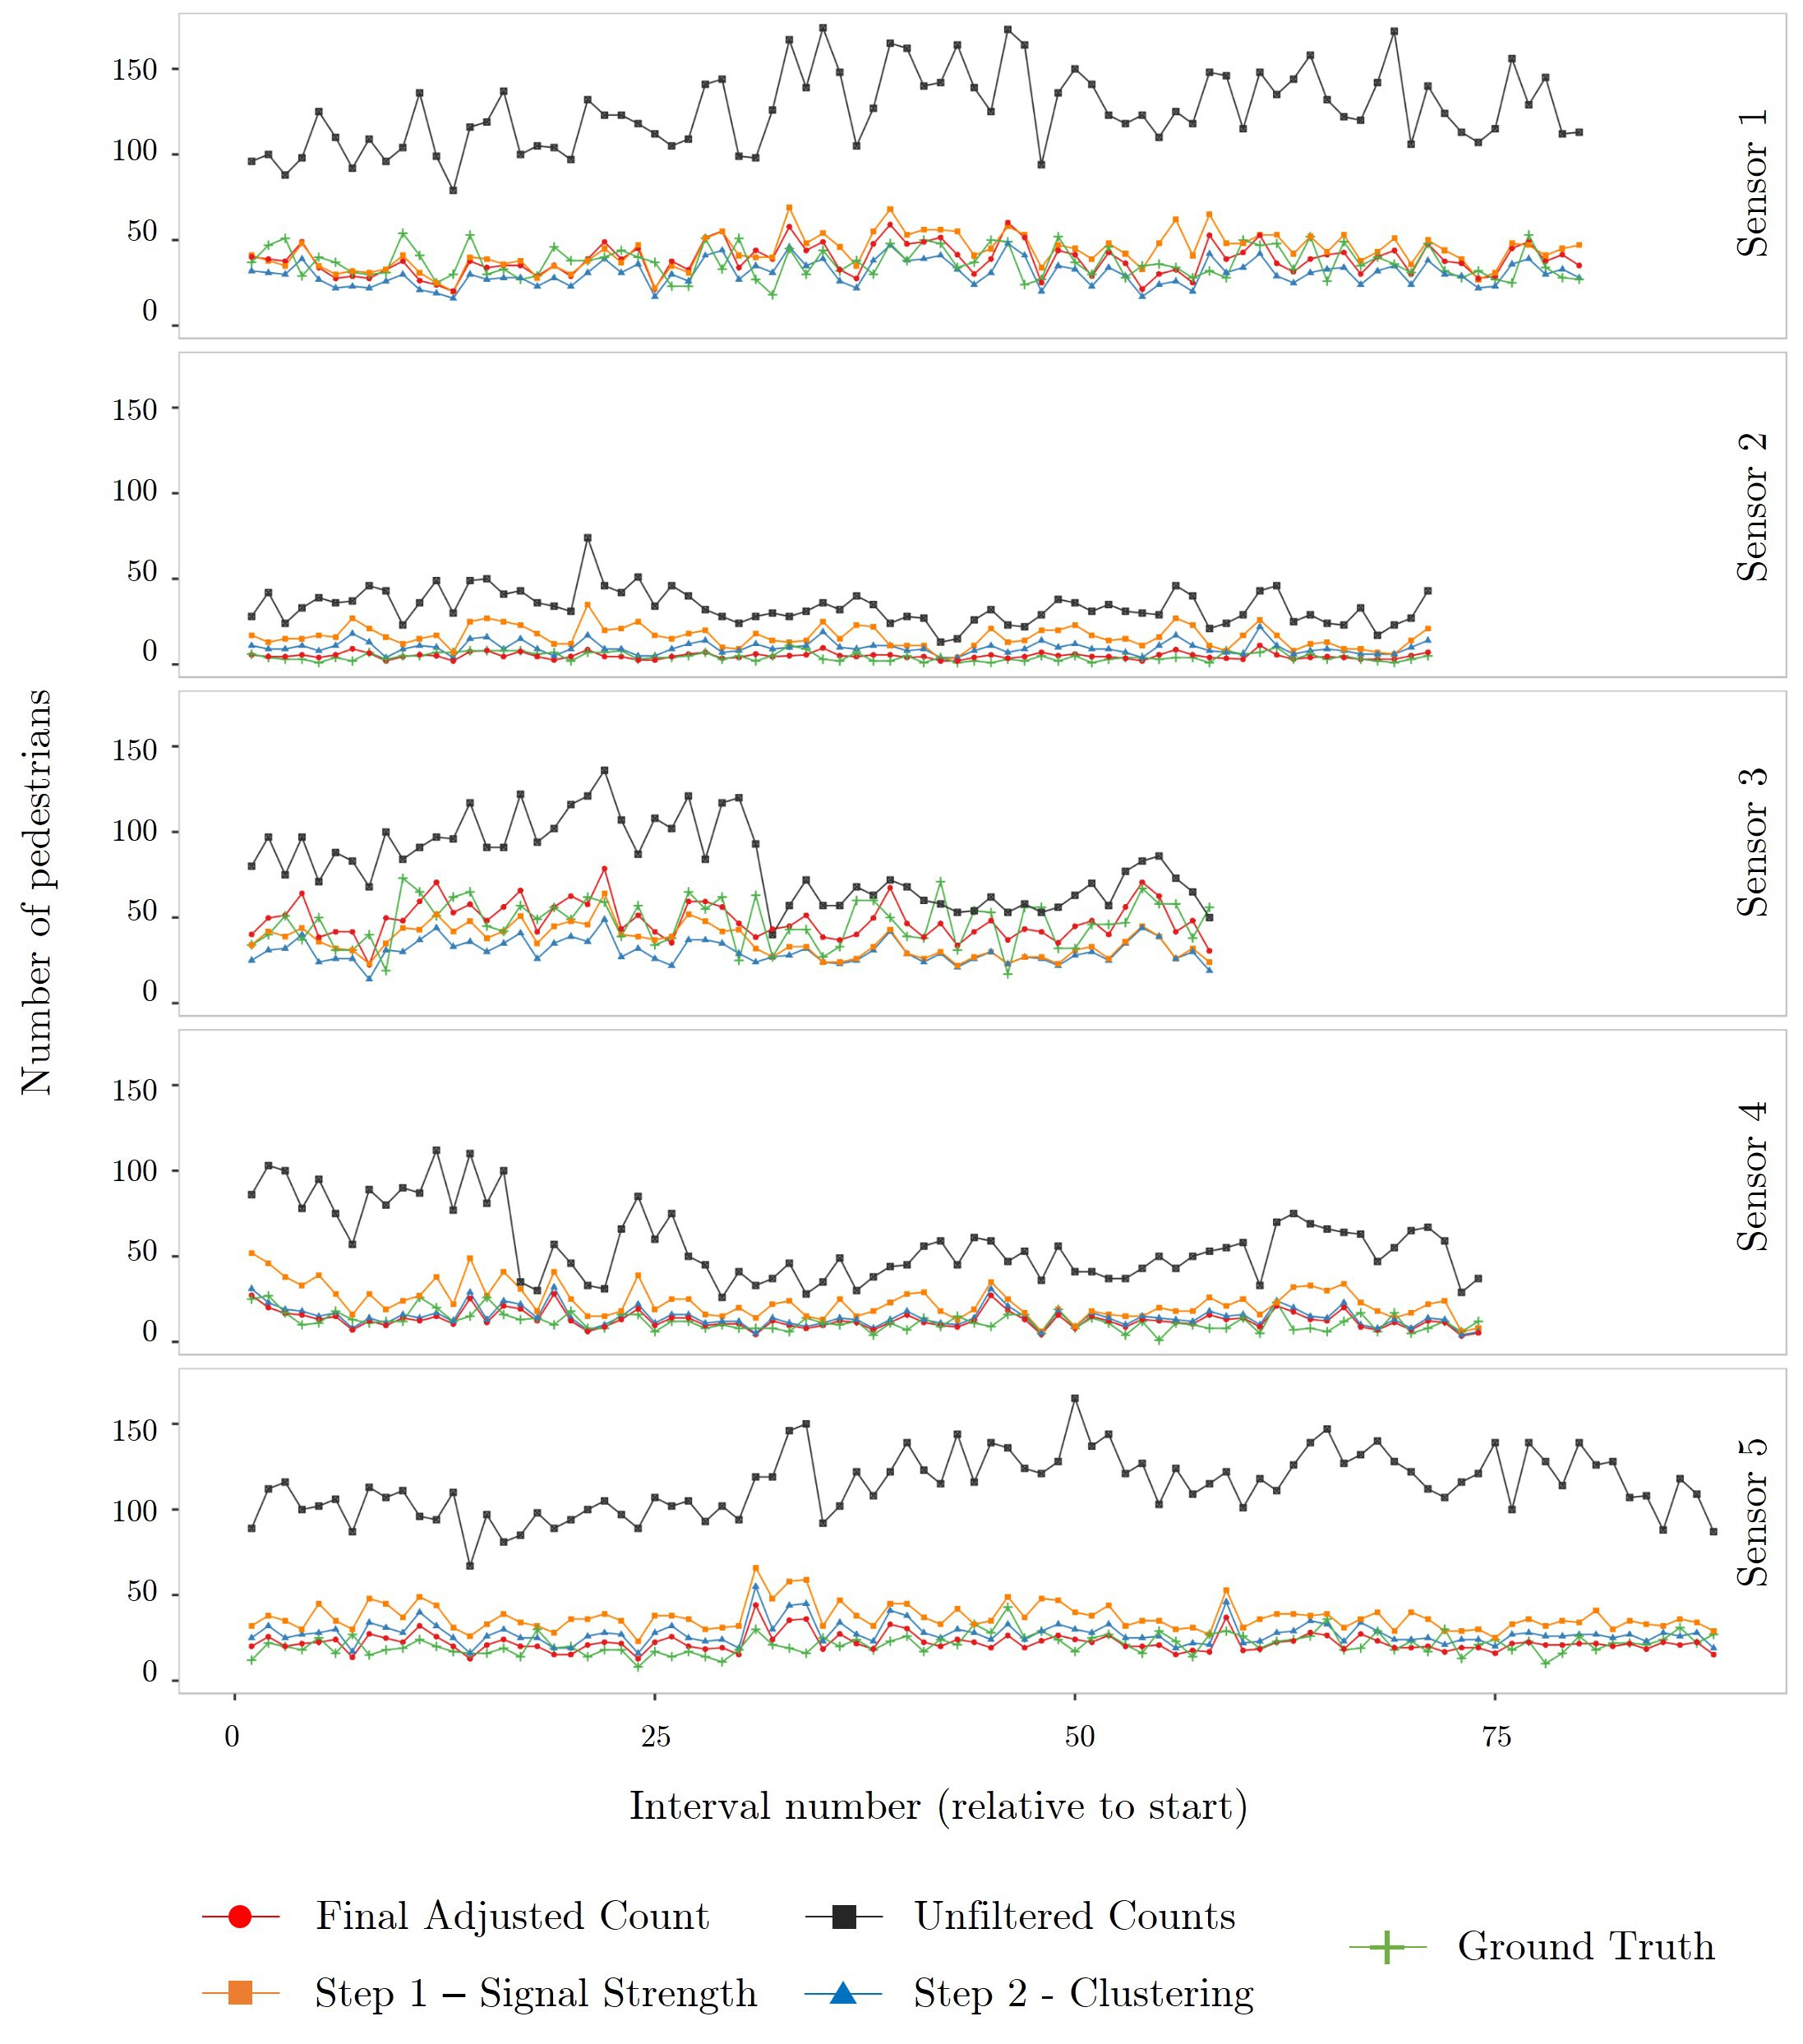
\includegraphics[trim=6 6 6 6, clip]{images/processing-pilot-results.jpg}
  \caption{A comparison of estimated footfall at pilot study locations during various stages of filtering with the actual manual counts.}
  \label{figure:processing:pilot:final}
\end{figure*}

%------------------------------------------------------------------------------%
\subsection{Smart Street Sensor Project}
%------------------------------------------------------------------------------%
In addition to solving problems arising due to privacy oriented decisions and figuring out methods to enhance Wi-Fi based analysis, one of the primary objectives of the research was to solve the problem faced by the Smart Street Sensor (SSS) project in respect of the explosion of MAC randomisation.
The number of probe requests and unique MAC addresses nearly tripled in one week in the autumn of 2017, which essentially made the data unusable and resulted in an extreme risk to the project’s feasibility.
The methodologies discussed above were perfect for the SSS project, and when implemented it would improve the project’s long term feasibility immensely.
However, being designed from a commercial point of view by the data partner, the SSS project’s implementation posed significant challenges in adapting to the methods as well.

\begin{itemize}
  \item \textit{Lack of data} - The data collected by the SSS project is optimised for transferring large amounts of data with the least possible cost. Hence, the project collects only the most important fields. For example, sequence number, information elements, SSID, etc. are not available in the dataset. 
  \item \textit{Aggregation} - To further optimise the size of the data transfer, the data points are aggregated at the device level every five minutes. Hence the time information has a resolution of 5 minutes and the signal strength of packets with same MAC addresses were summarised to either the maximum or minimum values observed in that interval.
  \item \textit{Cost} - When changing the design of the project, the major challenge faced was the cost associated with every change. For example, due to the size of the project, changing the amount of data transferred even marginally translated into a significant  increase in cost in terms of internet bandwidth, or the introduction of a large change in the project also involves a cost increase in terms of development, testing, deployment and testing.
\end{itemize}

The above challenges made the sequence number based clustering impossible to use with the data available through SSS sensors; as such, only the signal strength based filtering could be applied.
The signal strengths did not have the same granular information in them as the pilot study which may have greatly affected the output of the k-means algorithm.
Nevertheless, an attempt was made to use the signal strength based filtering on the data generated from the SSS sensors.
The data collected at the location where the pilot studies were conducted, along with manual counting, were extracted out of the SSS project and the filtering methodology was applied to the data.
Since we only have the minimum signal strength for all the probe requests that were compressed, the data were weighted using the total number of probes that constituted the aggregated packet.
Figure \ref{figure:processing:sss:signals} shows that the difference between the signal strength distribution measured by the sensors used in the pilot study and the corresponding sensors from Smart Street Sensor project.
It can be observed that the pilot study sensors collected data which shows a sharp change in the number of signal strengths after -70dBm comprising mostly of local MAC addresses, while the smart street sensors show a much more even distribution in both local and global MAC addresses.
Locations 4 and 3 are excellent examples indicating this difference in distribution, where the signal strengths of randomised probes were more normally distributed in the Smart Street Sensors than in their counterparts.
This was expected to pose a significant challenge to our filtering methodology, especially in locations with configurations similar to 4 and 3.

\begin{figure}
  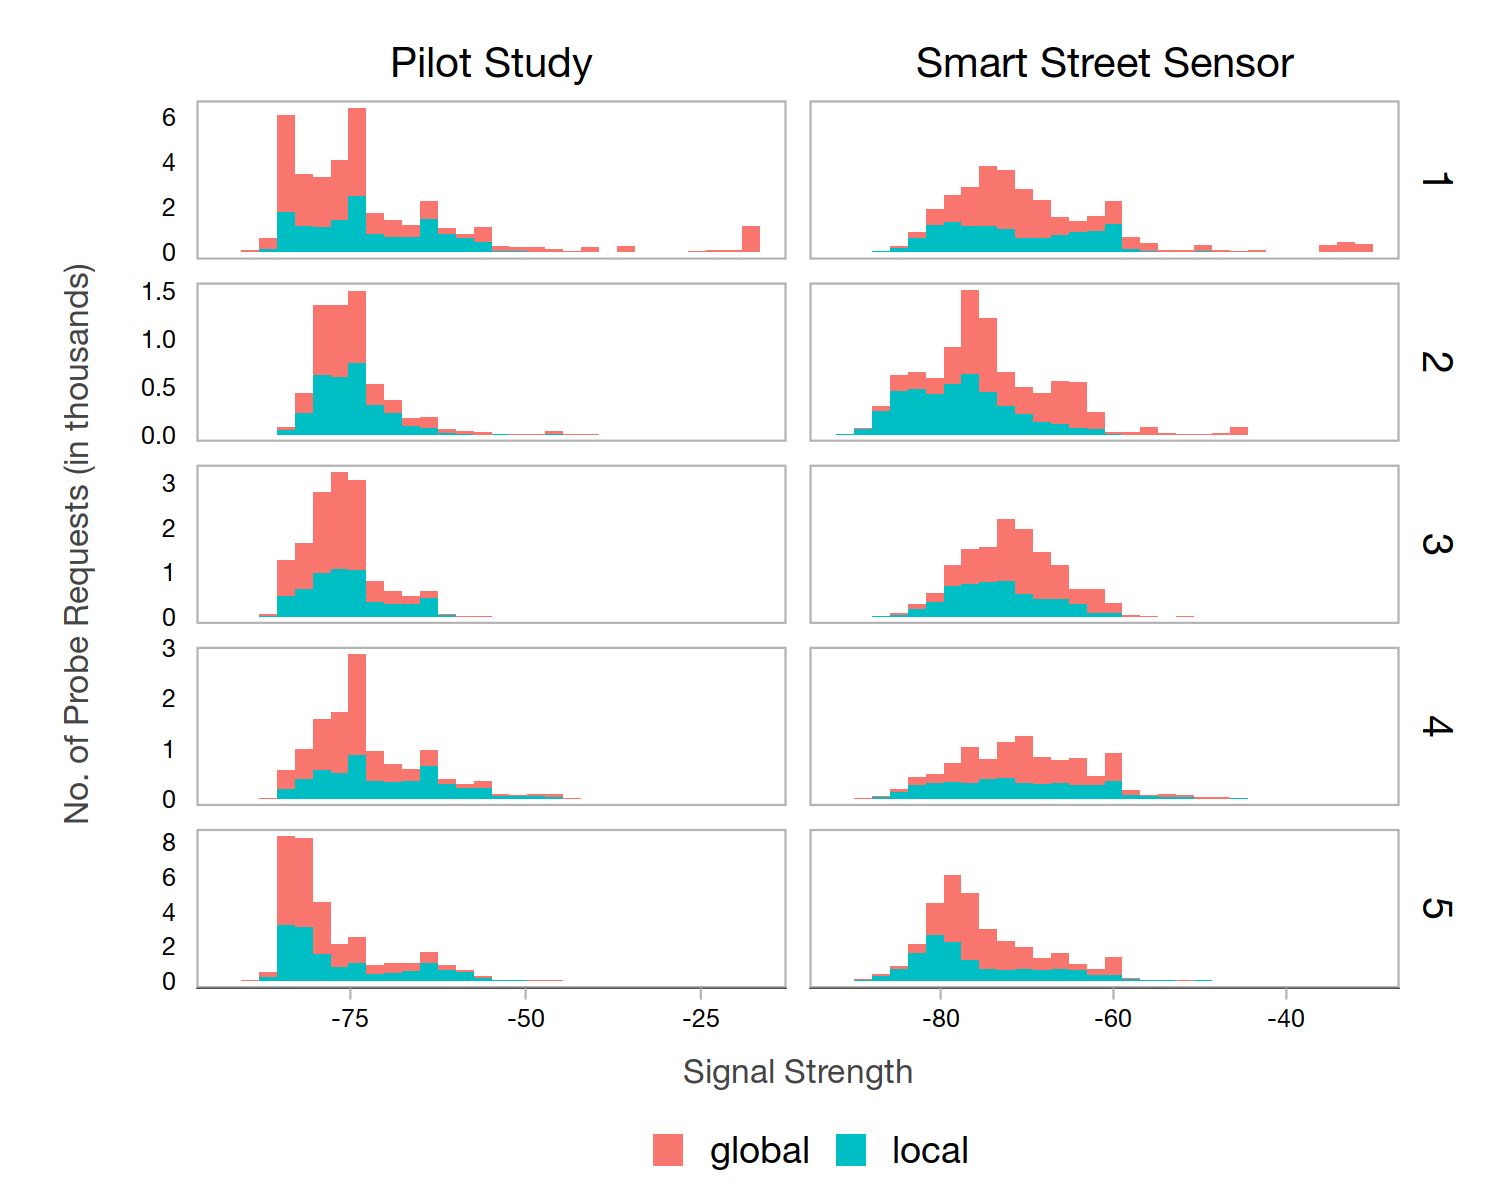
\includegraphics[trim={5 5 5 5}, clip]{images/processing-sss-signalsnew.png}
  \caption{Comparison between distribution of signal strengths in probe requests collected by }
  \label{figure:processing:sss:signals}
\end{figure}

There was an expectation that the change in the distribution might cause vast differences in the results from these two exercises.
However, when the probe requests collected by Smart Street Sensors were subject to filtering using the k-means algorithm and aggregated based on the MAC addresses after first removing the requests with low signal strength, the results were surprisingly close to what was reported by the pilot studies.
Figure \ref{figure:processing:sss:comparison} shows the results of the attempt to clean the smart street sensor data using the signal strength filtering technique, and compares them with the results of the pilot study.
It is important to note that the sequence number based clustering has not been carried out in either of the datasets as the sequence number is not available in the Smart Street Sensor data.
In general, it was observed that the results from the pilot study and the Smart Street Sensor project were close compared to the manual counts after the signal strength based filtering.
At Location 1, the pilot study sensor was massively over-counting on February 12 which could be attributed to a bug in the hardware: the additional Wi-Fi module which was installed for troubleshooting was generating probe requests in large amounts in response to very strong signal strengths.
This was fixed later and the next manual count performed on February 21 confirmed that the sensor was fixed.
At Location 2, the pilot study sensor resembled reality much more than the Smart Street Sensors, but footfall at this location was very low to begin with and both series showed similar trends and could be adjusted with a simple factor.
It was also observed that, similar to the results of the pilot study, Location 3 led to under-counting, Location 4 led to over-counting, but Location 5 showed the best results owing to the clean configuration of the sensor in relation to its surroundings.
Although the results are similar, they are still far from ground truth counts due to the MAC randomisation process and are also vulnerable to long-term changes, as shown in Figure \ref{figure:processing:error:random}.
This necessitates an alternative to the sequence number clustering for Smart Street Sensor data.

\begin{figure*}
  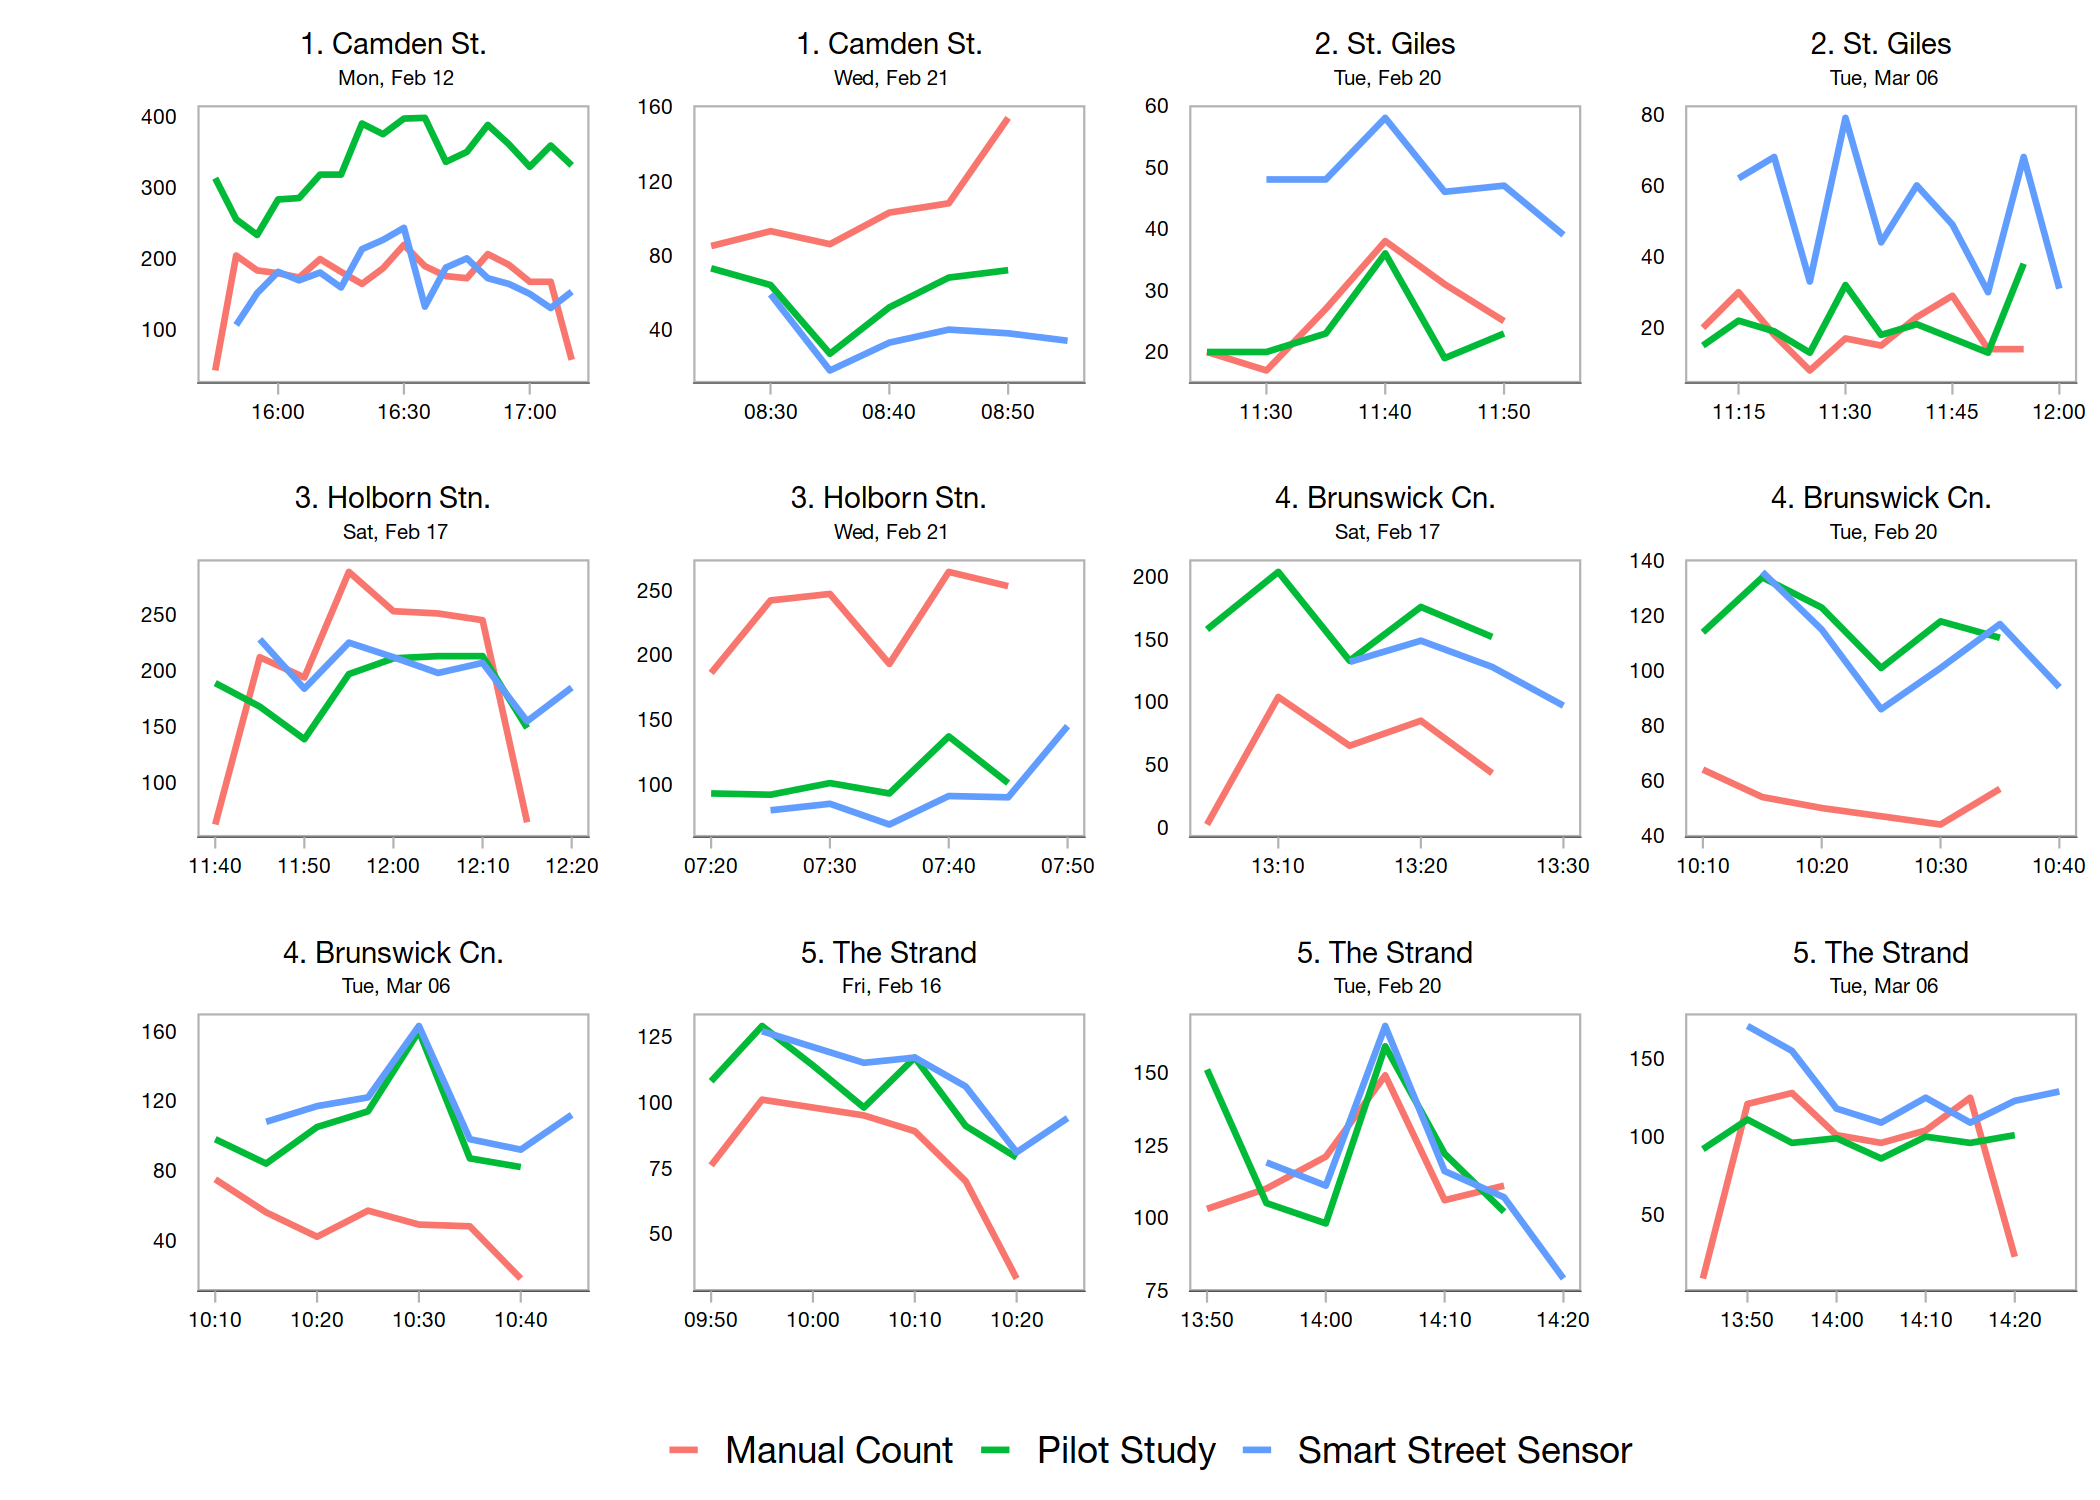
\includegraphics[trim={15 5 5 5}, clip]{images/processing-sss-compare.png}
  \caption{Comparison between the footfall estimates from Smart street sensor and pilot study after filtering probe requests of low signal strength along with manual footfall counts.}
  \label{figure:processing:sss:comparison}
\end{figure*}

\vspace{1.5em}\noindent\textit{Device to Probes Ratio}\vspace{0.5em}

While searching for an alternative to the sequence number algorithm with the limited data offered by the Smart street sensor, a much simpler approach was discovered.
This approach entailed found that the number of probe requests generated by devices which do not randomise their MAC address can be used to estimate the devices which do randomise them for a specific interval.
Assuming that, on average, all devices emit a certain number of probe requests in a given time interval, we can estimate the number of devices that are randomising as below,

\[Randomising\ devices = \frac{Non\ randomising\ devices}{Non\ randomised\ probes}\times{Randomised\ probes}\]

Although previous work on the probe request frequencies of different mobile devices demands scepticism over how well this method may work, the results were found to be encouraging.
In real world data, the rate of generation of probe requests between various mobile devices was not constant.
By encapsulating the problem in a small time interval - 5 minutes - and observing the corresponding non-randomising mobile phones, the behaviour of the randomising phones could be confidently estimated.
Moreover, if the randomisation techniques change in the future, the non-randomising phones should also alter, thus making such an approach robust against any future changes.
Figure \ref{figure:processing:sss:final} shows the methodology applied for data from locations across Cardiff.
The chart shows average weekly footfall estimated at each location before and after adjusting the number of randomised MAC addresses using the ‘compression’ ratio described above.

\begin{figure*}
  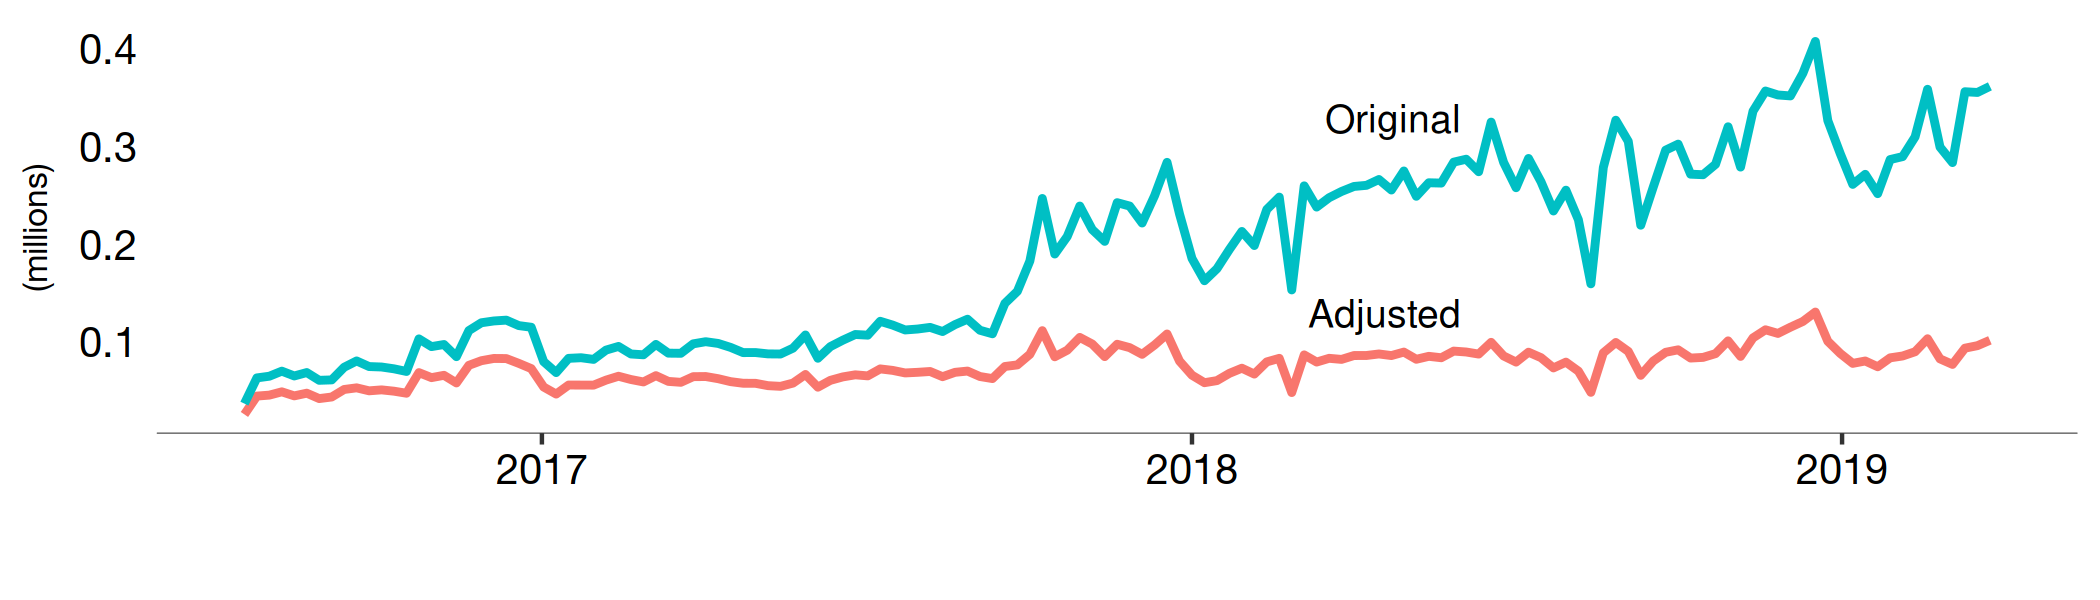
\includegraphics{images/processing-sss-final.png}
  \caption{The result of the adjustment using device to probes ratio in non-randomising devices shown through average weekly footfall estimates for locations in Cardiff.}
  \label{figure:processing:sss:final}
\end{figure*}

It was observed that, when adjusted, the resulting long term trend not only avoided the huge inflation experienced by the unadjusted estimate, but preserved the relative changes and trends and even showed seasonal variations.
The only expected disadvantage of this method is the adoption of randomisation techniques by manufacturers over the time.
Since the method depends on the number of devices that do not randomise their MAC address, when they decrease significantly in number, the method will fail.
But for the time being and for the data which have been collected over the past 3.5 years, when combined with filtering using signal strength and other adjustment methods described in section \ref{section:pipeline}, this method solves the uncertainties sufficiently.
Moreover, the method also potentially provides researchers with a reliable and sufficiently accurate estimation of footfall from the data collected by the Smart Street Sensors.

%------------------------------------------------------------------------------%
\subsection{Conclusions}
%------------------------------------------------------------------------------%

In this section, the uncertainties in the data collected through Wi-Fi - the ambiguity of the field of measurement and anonymisation of devices using MAC address randomisation - were discussed, alongside the extent to which these uncertainties affect the datasets.
Two techniques were proposed to tackle these sources of uncertainty.
The first technique involved using the strength of the signal reported in the probe requests to cluster the requests into ‘high’ and ‘low’ with the help of one dimensional clustering algorithms.
The second technique used the sequence numbers of the probe requests to group together probes generated by the same mobile devices using a graph based clustering algorithm.
The effectiveness of both of these techniques were tested against the data which were gathered in  Chapter \ref{chapter:collection}.

The data collected from the initial experiment on Oxford Street, London showed that filtering the probe requests using the signal strengths works very well.
In this case it reduced the MAPE from 435\% to 20\%.
This case study showed that k-means is the most suitable method of doing the clustering, while the threshold for this specific dataset is -70dBm similar to the others collected through initial experiments.
The case study also showed that fingerprinting unique mobile devices using sequence numbers is possible even in real world scenarios.
Through trial and error and a reference device, the ideal values for the parameters for the algorithm - time threshold($\alpha$) and sequence threshold($\beta$) are 60 and 16 respectively.

With the help of the pilot studies, it was also shown that signal strength based filtering does not always work efficiently everywhere.
The distribution of signal strengths were found to vary widely when  the sensors where installed in different configurations.
The counts were found to suffer from a lot of over-counting when there are multiple sources of noise located close to the sensors, and they also under-count considerably when used in a location where there are no significant sources of noise.
This emphasised the need for evaluating the site conditions and deploying manual calibration when utilising these techniques in real data.
The sequence number based fingerprinting was also demonstrated to work in all these locations.
This, along with signal strength and manual counts, reduced the error in the estimation from 470\% to 10\% in a ‘clean’ location with proper sensor configuration.

Unfortunately, the data from the Smart Street Sensor project was found to be insufficient to be able to effectively utilise these techniques, as the data were focused, aggregated, and prohibitively expensive to change.
Surprisingly, the signal strength data which were aggregated for five minutes for each MAC address by the minimum value, worked as well the detailed per packet data collected in the pilot study.
Although this, along with manual counting, can help in reducing the error, it does not solve the problems introduced by MAC randomisation, especially the long-term changes.
An alternate method using the ratio of probes to non-randomising devices was proposed and was found to be extremely efficient in eliminating the noise created by the randomisation.
The sample data from Cardiff showed that this method not only removes the massive increase in footfall estimates experienced since September 2017, but it also preserves the seasonal variations in the data thus enabling the data to be used for research into long-term phenomena.
